\documentclass[oneside,a4paper,14pt]{extreport}
\pdfminorversion=7

% Font tiếng Việt
\usepackage[T5]{fontenc}
\usepackage[utf8]{inputenc}
\DeclareTextSymbolDefault{\DH}{T1}

% Tài liệu tham khảo
\usepackage[
	sorting=nty,
	backend=biber]{biblatex}
\usepackage[unicode,hypertexnames=false]{hyperref} % Bookmark tiếng Việt
\usepackage{xurl} % Cho phép URL dài trong tài liệu tham khảo tự xuống dòng, tránh overfull hbox
\addbibresource{References/references.bib}

\makeatletter
\def\blx@maxline{77}
\makeatother

% Giảm cảnh báo Overfull \hbox nhỏ do LaTeX không tìm được điểm ngắt dòng đẹp
\emergencystretch=3em

% Chèn hình, các hình trong luận văn được để trong thư mục Images/
\usepackage{graphicx}
\graphicspath{ {Images/} }
\usepackage{pdfpages}

% Chèn và định dạng mã nguồn
\usepackage{listings}
\usepackage{color}
\definecolor{codegreen}{rgb}{0,0.6,0}
\definecolor{codegray}{rgb}{0.5,0.5,0.5}
\definecolor{codepurple}{rgb}{0.58,0,0.82}
\definecolor{backcolour}{rgb}{0.95,0.95,0.92}
\lstdefinestyle{mystyle}{
    backgroundcolor=\color{backcolour},   
    commentstyle=\color{codegreen},
    keywordstyle=\color{magenta},
    numberstyle=\tiny\color{codegray},
    stringstyle=\color{codepurple},
    basicstyle=\footnotesize,
    breakatwhitespace=false,         
    breaklines=true,                 
    captionpos=b,                    
    keepspaces=true,                 
    numbers=left,                    
    numbersep=5pt,                  
    showspaces=false,                
    showstringspaces=false,
    showtabs=false,                  
    tabsize=2
}
\lstset{style=mystyle}

% Chèn và định dạng mã giả
\usepackage{amsmath}
\usepackage{algorithm}
\usepackage[noend]{algpseudocode}
\makeatletter
\def\BState{\State\hskip-\ALG@thistlm}
\makeatother

% Bảng biểu
\usepackage{multirow}
\usepackage{array}
\newcolumntype{L}[1]{>{\raggedright\let\newline\\\arraybackslash\hspace{0pt}}m{#1}}
\newcolumntype{C}[1]{>{\centering\let\newline\\\arraybackslash\hspace{0pt}}m{#1}}
\newcolumntype{R}[1]{>{\raggedleft\let\newline\\\arraybackslash\hspace{0pt}}m{#1}}
% Cho phép ngắt dòng giữa các chuỗi dài không có khoảng trắng (tên bảng, tên cột CSDL...)
% để tránh tràn ô khi hiển thị trong bảng, ví dụ: \code{wallet_enhanced_transactions}
\usepackage{seqsplit}
\newcommand{\code}[1]{\texttt{\seqsplit{#1}}}
\usepackage{tabularx}
\usepackage{float}
\usepackage{placeins}

% Đổi tên mặc định
\renewcommand{\chaptername}{Chương}
\renewcommand{\figurename}{Hình}
\renewcommand{\tablename}{Bảng}
\renewcommand{\contentsname}{Mục lục}
\renewcommand{\listfigurename}{Danh sách hình}
\renewcommand{\listtablename}{Danh sách bảng}
\renewcommand{\appendixname}{Phụ lục}

% Ghi các danh sách vào mục lục sau khi tiêu đề đã tạo đúng hyperlink anchor.
\makeatletter
\patchcmd{\tableofcontents}{\@starttoc{toc}}{\addcontentsline{toc}{chapter}{\contentsname}\@starttoc{toc}}{}{}
\patchcmd{\listoffigures}{\@starttoc{lof}}{\addcontentsline{toc}{chapter}{\listfigurename}\@starttoc{lof}}{}{}
\patchcmd{\listoftables}{\@starttoc{lot}}{\addcontentsline{toc}{chapter}{\listtablename}\@starttoc{lot}}{}{}
\makeatother

\usepackage{longtable}

% Dãn dòng 1.5
\usepackage{setspace}
\onehalfspacing

% Thụt vào đầu dòng
\usepackage{indentfirst}

% Canh lề
\usepackage[
  top=30mm,
  bottom=25mm,
  left=30mm,
  right=20mm,
  includefoot]{geometry}
  
% Trang bìa
\usepackage{tikz}
\usetikzlibrary{calc}
\newcommand\HRule{\rule{\textwidth}{1pt}}

\begin{document}

\begin{titlepage}

\begin{center}
TRƯỜNG ĐẠI HỌC KHOA HỌC TỰ NHIÊN\\
\textbf{KHOA CÔNG NGHỆ THÔNG TIN}\\[2cm]


{ \Large \bfseries Dương Hoàng Hồng Phúc - Lê Võ Minh Phương - Nguyễn Mạnh Phương - Lê Minh Quân - Võ Hoàng Anh Quân - Nguyễn Minh Thiện\\[2cm] } 

{ \Large \bfseries XÂY DỰNG HỆ THỐNG PHÂN TÍCH DỮ
LIỆU ON-CHAIN SOLANA VÀ TRỰC QUAN
HÓA HÀNH VI VÍ BLOCKCHAIN \\[3cm]} 


\large THỰC TẬP DỰ ÁN TỐT NGHIỆP CỬ NHÂN\\
\large CHƯƠNG TRÌNH CHÍNH QUY\\


\begin{tikzpicture}[remember picture, overlay]
  \draw[line width = 2pt] ($(current page.north west) + (2cm,-2cm)$) rectangle ($(current page.south east) + (-1.5cm,2cm)$);
\end{tikzpicture}

\vfill
Tp. Hồ Chí Minh, tháng 07/2026

\end{center}

\pagebreak



\begin{center}

TRƯỜNG ĐẠI HỌC KHOA HỌC TỰ NHIÊN\\
\textbf{KHOA CÔNG NGHỆ THÔNG TIN}\\[2cm]


{\large \bfseries Dương Hoàng Hồng Phúc - 22120271\\
            Lê Võ Minh Phương - 22120286\\
            Nguyễn Mạnh Phương - 22120287\\
            Lê Minh Quân - 22120290\\
            Võ Hoàng Anh Quân - 22120293\\
            Nguyễn Minh Thiện - 22120344\\} 


{ \Large \bfseries XÂY DỰNG HỆ THỐNG PHÂN TÍCH DỮ
LIỆU ON-CHAIN SOLANA VÀ TRỰC QUAN
HÓA HÀNH VI VÍ BLOCKCHAIN \\[2cm]}  


\large THỰC TẬP DỰ ÁN TỐT NGHIỆP CỬ NHÂN\\
\large CHƯƠNG TRÌNH CHÍNH QUY\\[1.8cm]

\textbf{GIẢNG VIÊN HƯỚNG DẪN}\\
ThS. Phạm Nguyễn Sơn Tùng\\
ThS. Hồ Tuấn Thanh\\


\begin{tikzpicture}[remember picture, overlay]
  \draw[line width = 2pt] ($(current page.north west) + (2cm,-2cm)$) rectangle ($(current page.south east) + (-1.5cm,2cm)$);
\end{tikzpicture}

\vfill
Tp. Hồ Chí Minh, tháng 07/2026

\end{center}

\end{titlepage}


\pagenumbering{roman}

\chapter*{Lời cam đoan}
\label{reassurances}

Nhóm chúng em xin cam đoan đồ án tốt nghiệp ``Xây dựng hệ thống phân tích dữ liệu on-chain Solana và trực quan hóa hành vi ví blockchain'' là kết quả nghiên cứu, thiết kế và phát triển của tập thể nhóm dưới sự hướng dẫn của ThS. Phạm Nguyễn Sơn Tùng và ThS. Hồ Tuấn Thanh.

Các nội dung, số liệu và kết quả trình bày trong báo cáo được tổng hợp từ quá trình thực hiện đề tài. Tài liệu, dữ liệu và ý tưởng từ các tác giả, tổ chức hoặc dịch vụ bên ngoài đều được ghi nhận và trích dẫn theo quy định học thuật. Nhóm chúng em chịu trách nhiệm trước Hội đồng và Nhà trường về nội dung của báo cáo này.


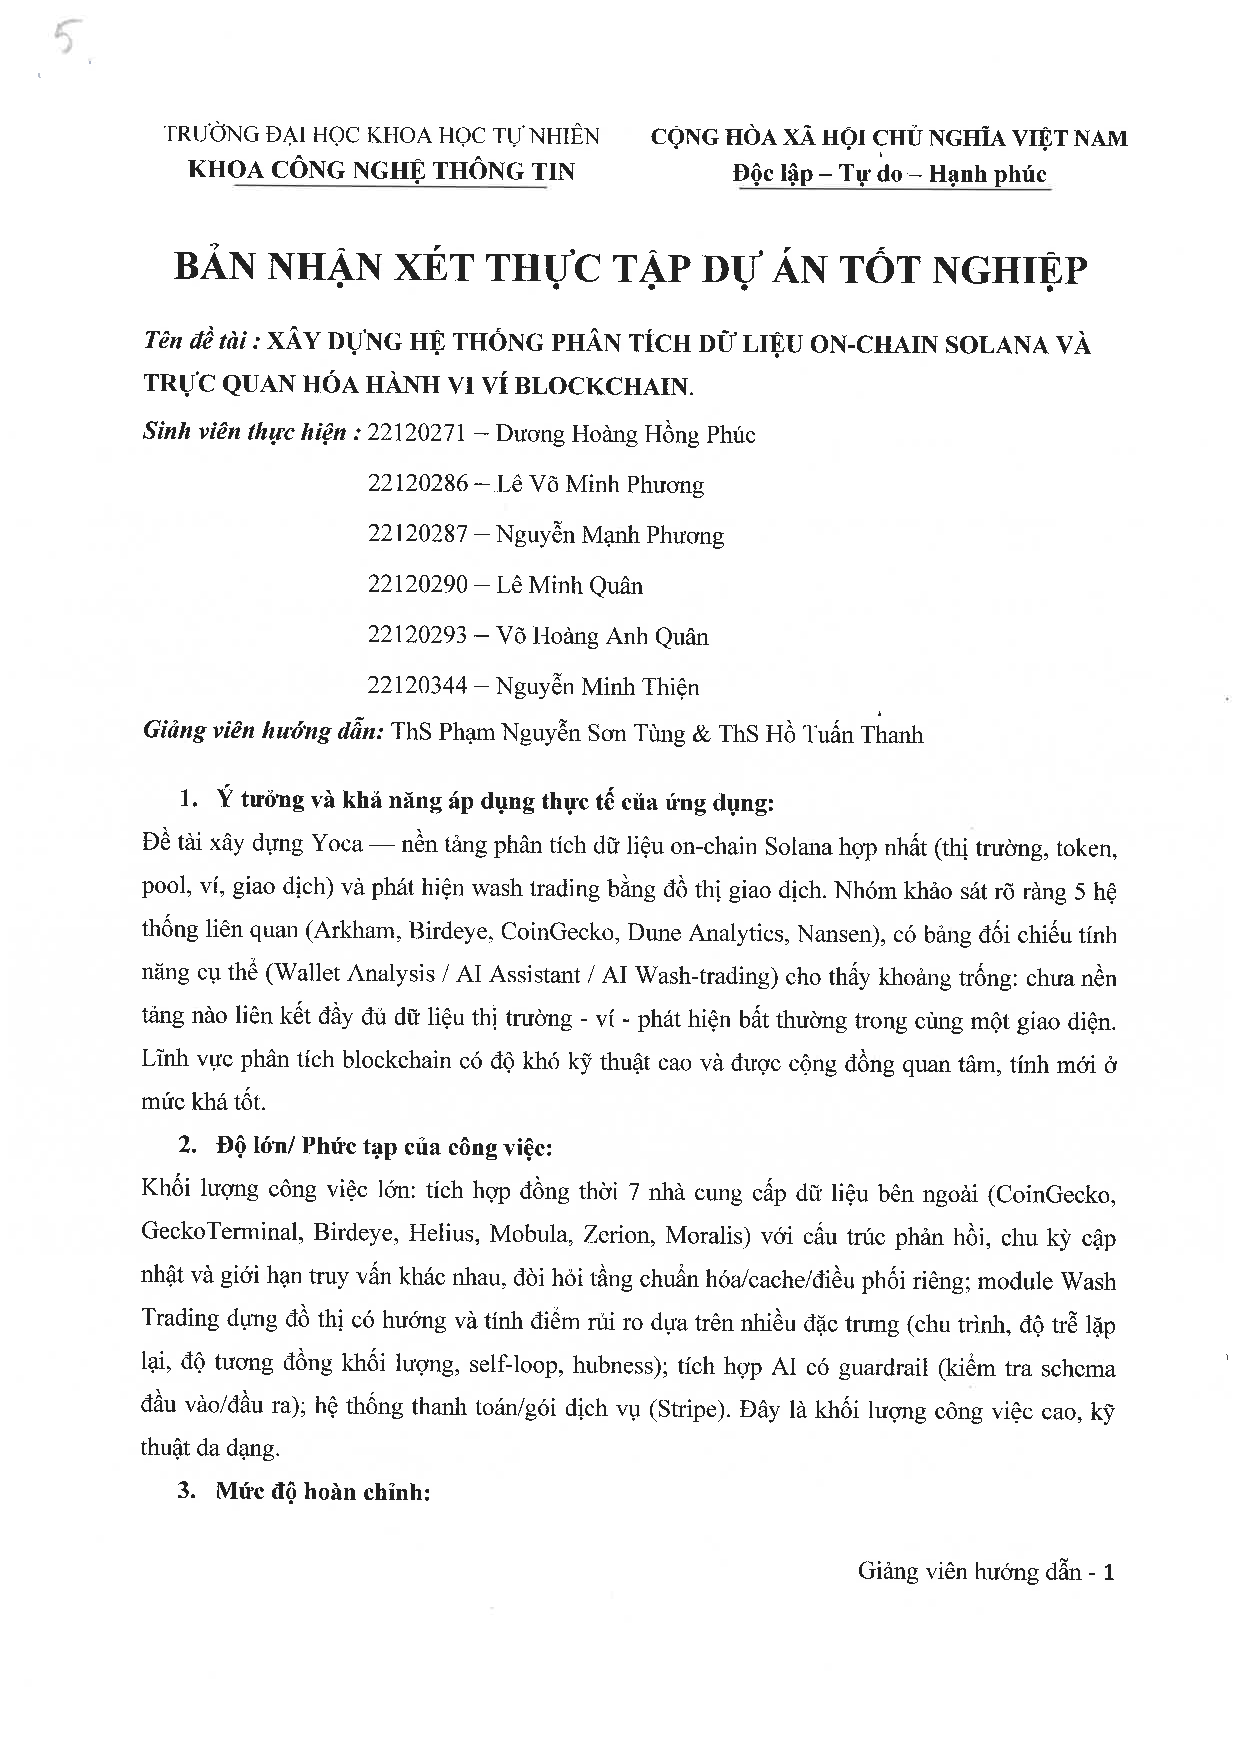
\includepdf[pages=1-3]{25D2-DA-KTPM13.pdf}


\includepdf[
    pages=4,
    pagecommand={
        \thispagestyle{empty}
        \phantomsection
        \addcontentsline{toc}{chapter}{Nhận xét phản biện}
    }
]{25D2-DA-KTPM13.pdf}
\includepdf[
    pages=5
]{25D2-DA-KTPM13.pdf}


\chapter*{Lời cảm ơn}
\label{thanks}

Nhóm chúng em xin chân thành cảm ơn ThS. Phạm Nguyễn Sơn Tùng và ThS. Hồ Tuấn Thanh đã định hướng, góp ý và đồng hành cùng nhóm trong suốt quá trình thực hiện đồ án. Những trao đổi với quý Thầy giúp nhóm nhìn bài toán có hệ thống hơn, từ xác định phạm vi, lựa chọn giải pháp kỹ thuật đến tổ chức và trình bày kết quả.

Nhóm chúng em trân trọng cảm ơn Ban Giám hiệu Trường Đại học Khoa học Tự nhiên, Đại học Quốc gia Thành phố Hồ Chí Minh, cùng quý Thầy, Cô Khoa Công nghệ Thông tin đã tạo môi trường học tập và cung cấp những kiến thức nền tảng cần thiết để nhóm triển khai đề tài.

Nhóm cũng ghi nhận sự hỗ trợ của các dịch vụ và cộng đồng mã nguồn mở. CoinGecko, GeckoTerminal, Birdeye, Helius, Mobula, Zerion và Moralis cung cấp dữ liệu cho các miền thị trường, token, pool, ví và giao dịch; Google Gemini hỗ trợ chức năng diễn giải; Stripe phục vụ thanh toán; Render và Supabase cung cấp hạ tầng triển khai. React, Hono, PostgreSQL, Drizzle ORM và ECharts là những công nghệ quan trọng trong quá trình xây dựng sản phẩm.

Sau cùng, nhóm chúng em cảm ơn gia đình, bạn bè và tất cả thành viên trong nhóm đã luôn hỗ trợ, chia sẻ trách nhiệm và duy trì tinh thần hợp tác trong suốt quá trình thực hiện đề tài.



\includepdf[
    pages=1,
    pagecommand={
        \thispagestyle{empty}
        \phantomsection
        \addcontentsline{toc}{chapter}{Đề cương chi tiết}
    }
]{Appendix/proposal.pdf}

\includepdf[
    pages=2-
]{Appendix/proposal.pdf}


\tableofcontents

\listoffigures

\listoftables

\chapter*{Bảng thuật ngữ}
\addcontentsline{toc}{chapter}{Bảng thuật ngữ}
\label{glossary}

Báo cáo sử dụng một số thuật ngữ chuyên ngành thuộc lĩnh vực blockchain, tài chính số và kiến trúc phần mềm. Phần lớn các thuật ngữ này đã được dịch hoặc diễn giải bằng tiếng Việt ngay trong nội dung từng chương; bảng dưới đây tổng hợp lại những thuật ngữ thông dụng nhất để tiện tra cứu trong suốt quá trình đọc báo cáo.

\renewcommand{\arraystretch}{1.3}
\small
\begin{longtable}{|L{3.8cm}|L{11.2cm}|}
\hline
\textbf{Thuật ngữ} & \textbf{Giải thích} \\
\hline
\endfirsthead

\multicolumn{2}{c}{\textit{(Bảng thuật ngữ - tiếp theo)}} \\
\hline
\textbf{Thuật ngữ} & \textbf{Giải thích} \\
\hline
\endhead

\hline
\multicolumn{2}{r}{\textit{(còn tiếp ở trang sau)}} \\
\endfoot

\hline
\endlastfoot

Adapter & Lớp trung gian trong backend, chuyển dữ liệu từ định dạng riêng của một nhà cung cấp bên ngoài sang định dạng nội bộ thống nhất của hệ thống. \\
\hline

AI Assistant (Trợ lý AI) & Thành phần sử dụng mô hình ngôn ngữ lớn để tóm tắt và diễn giải dữ liệu ví, token hoặc tín hiệu wash trading dựa trên ngữ cảnh đã được hệ thống chuẩn hóa. \\
\hline

API (Application Programming Interface) & Giao diện lập trình ứng dụng, tập hợp quy tắc để các thành phần phần mềm giao tiếp và trao đổi dữ liệu với nhau. \\
\hline

Backend & Phần máy chủ của ứng dụng, đảm nhiệm xác thực, xử lý nghiệp vụ, truy cập cơ sở dữ liệu và tích hợp với các nhà cung cấp dữ liệu bên ngoài. \\
\hline

Blockchain & Chuỗi khối, một dạng sổ cái phân tán lưu trữ dữ liệu giao dịch một cách công khai, có thể kiểm chứng và khó bị thay đổi. \\
\hline

Cache / Caching (Lưu trữ đệm) & Cơ chế lưu lại dữ liệu đã truy xuất để tái sử dụng cho các lần yêu cầu sau, giúp giảm số lượt gọi đến nhà cung cấp bên ngoài và cải thiện tốc độ phản hồi. \\
\hline

DeFi (Decentralized Finance) & Tài chính phi tập trung, các dịch vụ tài chính như cho vay, giao dịch hay tạo thanh khoản được vận hành trực tiếp trên blockchain, không qua trung gian truyền thống. \\
\hline

DEX (Decentralized Exchange) & Sàn giao dịch phi tập trung, nơi người dùng hoán đổi token trực tiếp thông qua hợp đồng thông minh thay vì thông qua một đơn vị trung gian. \\
\hline

Endpoint & Một địa chỉ cụ thể trong API mà frontend hoặc dịch vụ khác gửi yêu cầu đến để lấy hoặc gửi dữ liệu. \\
\hline

ERD (Entity Relationship Diagram) & Sơ đồ thực thể mối quan hệ, mô tả các nhóm bảng chính và mối liên hệ giữa chúng trong cơ sở dữ liệu. \\
\hline

Frontend & Phần giao diện người dùng của ứng dụng, đảm nhiệm hiển thị dữ liệu, tiếp nhận thao tác và trực quan hóa thông tin. \\
\hline

Full-stack & Kiến trúc ứng dụng bao gồm cả phần giao diện (frontend) và phần máy chủ (backend) được phát triển trong cùng một hệ thống. \\
\hline

GCN / GAT / GraphSAGE & Tên ba kiến trúc mạng nơ-ron đồ thị. Trong Yoca, các tên này được dùng cho ba cấu hình trọng số heuristic lấy cảm hứng từ GNN; hệ thống không sử dụng mô hình GNN đã huấn luyện. \\
\hline

Holder & Địa chỉ ví đang nắm giữ một loại token nhất định. \\
\hline

Heuristic & Quy tắc suy luận thực nghiệm dùng để đưa ra kết quả gần đúng khi dữ liệu không cung cấp trực tiếp thông tin cần thiết; kết quả cần được đối chiếu và không bảo đảm đúng cho mọi trường hợp. \\
\hline

Localization (Bản địa hóa) & Việc điều chỉnh chuỗi giao diện, số, ngày giờ, tiền tệ và cách trình bày cho một ngôn ngữ hoặc khu vực cụ thể; Yoca hiện hỗ trợ locale tiếng Anh và tiếng Việt. \\
\hline

LLM (Large Language Model) & Mô hình ngôn ngữ lớn, được sử dụng để diễn giải các chỉ số đã tính toán thành nội dung bằng ngôn ngữ tự nhiên. \\
\hline

Monolith & Kiến trúc backend được triển khai như một ứng dụng thống nhất duy nhất, nhưng bên trong được chia thành nhiều lớp và miền nghiệp vụ riêng biệt. \\
\hline

Monorepo & Cách tổ chức mã nguồn trong đó nhiều thành phần của dự án như frontend, backend và tài liệu kỹ thuật cùng nằm trong một kho mã nguồn duy nhất. \\
\hline

On-chain & Dữ liệu hoặc hoạt động được ghi nhận trực tiếp trên blockchain và có thể kiểm tra từ lịch sử của mạng lưới. \\
\hline

ORM (Object-Relational Mapping) & Công cụ ánh xạ giữa cấu trúc bảng trong cơ sở dữ liệu quan hệ với các đối tượng trong mã nguồn, giúp truy vấn dữ liệu an toàn hơn về kiểu dữ liệu. \\
\hline

PnL (Profit and Loss) & Lãi/lỗ, chỉ số phản ánh kết quả tăng hoặc giảm giá trị tài sản của một ví theo thời gian. \\
\hline

Pool (Pool thanh khoản) & Quỹ thanh khoản chứa cặp tài sản, dùng để thực hiện giao dịch hoán đổi trên các sàn phi tập trung. \\
\hline

Provider (Nhà cung cấp dữ liệu) & Nhà cung cấp dữ liệu bên thứ ba, ví dụ Helius, CoinGecko hoặc Birdeye, nơi hệ thống truy xuất dữ liệu on-chain hoặc dữ liệu thị trường. \\
\hline

Rate limit (Giới hạn truy vấn) & Giới hạn về số lượng hoặc tần suất yêu cầu mà một API cho phép trong một khoảng thời gian nhất định. \\
\hline

Request coalescing & Cơ chế gộp nhiều yêu cầu dữ liệu giống nhau phát sinh đồng thời thành một lần gọi duy nhất đến nhà cung cấp. \\
\hline

Schema (Lược đồ dữ liệu) & Mô tả cấu trúc các bảng, cột và mối quan hệ trong cơ sở dữ liệu. \\
\hline

Tiêu chí chấp nhận (Acceptance Criteria) & Điều kiện cụ thể dùng để xác định một chức năng hoặc luồng sử dụng đã đáp ứng yêu cầu đặt ra hay chưa. \\
\hline

Swap & Giao dịch hoán đổi trực tiếp giữa hai loại token thông qua giao thức phi tập trung. \\
\hline

Token & Đơn vị tài sản số được phát hành và giao dịch trên blockchain, có thể đại diện cho tiền mã hóa, quyền sở hữu hoặc một loại tài sản khác. \\
\hline

TTL (Time To Live) & Khoảng thời gian một dữ liệu cache được xem là còn hợp lệ trước khi hệ thống cần cập nhật lại từ nhà cung cấp. \\
\hline

Use Case (Tình huống sử dụng) & Mô tả một tương tác cụ thể giữa tác nhân, có thể là người dùng hoặc hệ thống bên ngoài, với hệ thống đang xây dựng. \\
\hline

Wallet (Ví) & Địa chỉ dùng để lưu trữ, quản lý và thực hiện giao dịch tài sản số trên blockchain. \\
\hline

Wash trading & Hành vi giao dịch được phối hợp thực hiện nhằm tạo ra khối lượng hoặc mức độ hoạt động giả cho một tài sản. \\
\hline

Watchlist (Danh sách theo dõi) & Danh sách token hoặc ví được người dùng lưu lại để tiện theo dõi. \\
\hline

Webhook & Cơ chế cho phép một dịch vụ tự động gửi dữ liệu đến một địa chỉ đã đăng ký ngay khi có sự kiện xảy ra, thay vì phải chủ động truy vấn liên tục. \\
\hline

\end{longtable}
\normalsize

\chapter*{Tóm tắt}
\label{summary}

Dữ liệu trên Solana được phân bố giữa nhiều dịch vụ chuyên biệt về thị trường, token, pool thanh khoản, ví và giao dịch, khiến người dùng gặp khó khăn khi tổng hợp thông tin. Đề tài hướng đến xây dựng Yoca, một nền tảng web hỗ trợ khám phá thị trường, phân tích token, pool, ví và trực quan hóa hành vi giao dịch trên Solana. Hệ thống được phát triển theo kiến trúc full-stack TypeScript với React và Vite ở phía giao diện, Hono ở phía máy chủ, PostgreSQL và Drizzle ORM ở lớp dữ liệu. Các nguồn CoinGecko, GeckoTerminal, Birdeye, Helius, Mobula, Zerion và Moralis được tích hợp; dữ liệu bên ngoài được kiểm tra, chuẩn hóa và lưu đệm trước khi cung cấp cho các chức năng phân tích. Yoca kết hợp biểu đồ tài chính, lịch sử giao dịch, danh mục tài sản và chỉ số lãi/lỗ để phân tích ví. Mô-đun Wash Trading sử dụng đồ thị có hướng cùng các đặc trưng về chu trình, thời gian, lượng token và cấu trúc liên kết để nhận diện những hoạt động đáng chú ý. Hệ thống còn hỗ trợ so sánh ví, watchlist, cảnh báo và trợ lý AI. Kết quả kiểm thử ghi nhận 178/178 trường hợp phía client và 204/204 trường hợp phía server đạt yêu cầu; hệ thống được triển khai trên Render và sử dụng cơ sở dữ liệu Supabase. Kết quả đề tài tạo ra một quy trình phân tích on-chain liền mạch, giúp người dùng tiếp cận dữ liệu Solana có hệ thống và cung cấp nền tảng để mở rộng nghiên cứu về hành vi ví và giao dịch bất thường.

\textbf{Từ khóa:} Solana, phân tích on-chain, tích hợp dữ liệu, phân tích ví, PnL, wash trading, trí tuệ nhân tạo.


\clearpage

\pagenumbering{arabic}

\chapter{Giới thiệu}
\label{Chapter1}

Chương này trình bày bối cảnh của tài chính phi tập trung (DeFi) và những rào cản mà người dùng gặp phải khi tiếp cận, phân tích dữ liệu trên hệ sinh thái Solana. Trên cơ sở nhận diện các vấn đề thực tiễn và khoảng trống của những giải pháp hiện có, chương xác định mục tiêu, đối tượng, phạm vi ứng dụng và hướng tiếp cận của nền tảng Yoca, đồng thời khái quát những đóng góp chính của đề tài.

\section{Đặt vấn đề}
\label{sec:dat_van_de}

\subsection{Ngữ cảnh và vấn đề thực tiễn}

Trong những năm gần đây, công nghệ blockchain đã trở thành nền tảng cho sự phát triển của nhiều ứng dụng tài chính phi tập trung. Trong đó, Solana là một hệ sinh thái đáng chú ý nhờ khả năng xử lý giao dịch với thông lượng cao và chi phí tương đối thấp, tạo điều kiện cho sự hình thành của nhiều token, pool thanh khoản, sàn giao dịch phi tập trung và các ứng dụng DeFi.

Cùng với sự phát triển đó, khối lượng dữ liệu được ghi nhận trên mạng lưới ngày càng gia tăng. Mặc dù dữ liệu on-chain có tính công khai và có thể kiểm chứng, việc khai thác và diễn giải dữ liệu vẫn tương đối phức tạp. Một giao dịch có thể liên quan đến nhiều tài khoản, nhiều lần chuyển token và nhiều chương trình khác nhau. Để hiểu đầy đủ bối cảnh của một token hoặc ví, người dùng thường phải kết hợp dữ liệu từ nền tảng theo dõi thị trường, công cụ phân tích ví, trình khám phá blockchain và các nguồn thông tin khác nhau.

Sự phân tán giữa các công cụ khiến quá trình phân tích dễ bị gián đoạn và đòi hỏi người dùng phải có kiến thức kỹ thuật nhất định. Các chỉ số về giá, thanh khoản, phân bố holder, lịch sử giao dịch, biến động số dư và dòng tiền thường được trình bày riêng lẻ, trong khi mối liên hệ giữa token, pool, ví và giao dịch chưa được thể hiện trong một luồng phân tích thống nhất.

Bên cạnh đó, dữ liệu thị trường có thể chịu ảnh hưởng bởi wash trading, tức các hoạt động giao dịch mang tính phối hợp nhằm tạo ra cảm nhận sai lệch về khối lượng hoặc mức độ hoạt động của một tài sản. Nếu chỉ quan sát những chỉ số tổng hợp, người dùng khó nhận biết cấu trúc giao dịch và mối quan hệ giữa các ví đứng sau những biến động này.

\subsection{Tính cấp thiết và độ khó của bài toán}

Bài toán xây dựng một nền tảng phân tích dữ liệu Solana bao gồm việc tổng hợp, hiển thị và duy trì dữ liệu nhất quán theo thời gian. Dữ liệu blockchain phát sinh liên tục, trong khi mỗi nhà cung cấp có phạm vi bao phủ, chu kỳ cập nhật, cấu trúc phản hồi và chính sách giới hạn truy vấn khác nhau.

Một trang phân tích token hoặc ví có thể cần đồng thời nhiều nhóm dữ liệu như thông tin nhận diện, giá, biểu đồ lịch sử, pool, holder, danh mục tài sản, swap và chuyển token. Nếu các yêu cầu này được gửi trực tiếp và lặp lại đến nhà cung cấp, hệ thống dễ gặp giới hạn truy vấn, làm tăng thời gian phản hồi và ảnh hưởng đến trải nghiệm sử dụng.

Đối với dữ liệu lịch sử, hệ thống cần có khả năng tái sử dụng phần dữ liệu đã được đồng bộ khi người dùng thay đổi khoảng thời gian phân tích. Việc định giá danh mục ví tại một thời điểm trong quá khứ còn yêu cầu tái dựng số dư token và kết hợp với dữ liệu giá tương ứng. Những token mới, có thanh khoản thấp hoặc thiếu dữ liệu giá lịch sử cần được xử lý thận trọng để tránh tạo ra kết quả thiếu căn cứ.

Bài toán phát hiện wash trading cũng có độ phức tạp riêng. Một giao dịch đơn lẻ thường không đủ để phản ánh dấu hiệu bất thường; quá trình phân tích cần xem xét quan hệ giữa nhiều ví, hướng luân chuyển token, mức độ lặp lại về thời gian và số lượng, cũng như sự xuất hiện của các chu trình giao dịch. Vì vậy, dữ liệu được đặt trong bối cảnh của mạng lưới giao dịch để làm rõ mối liên hệ giữa các bản ghi riêng lẻ.

Ngoài ra, việc tích hợp trí tuệ nhân tạo vào phân tích dữ liệu tài chính cần bảo đảm nội dung diễn giải có cơ sở đối chiếu. Mô hình ngôn ngữ cần sử dụng dữ liệu đã được hệ thống tính toán và chuẩn hóa, trong khi bảng, biểu đồ và giao dịch nguồn vẫn đóng vai trò là căn cứ chính của quá trình phân tích.

\subsection{Hạn chế của các giải pháp hiện tại}

Thị trường hiện có nhiều nền tảng hỗ trợ theo dõi và phân tích dữ liệu blockchain như Arkham Intelligence, Birdeye, CoinGecko, Dune Analytics và Nansen. Mỗi nền tảng có thế mạnh riêng, từ dữ liệu giá, khối lượng và thanh khoản đến truy vết dòng tiền, gắn nhãn ví hoặc xây dựng dashboard truy vấn dữ liệu.

Tuy nhiên, khi xét trong phạm vi của đề tài, vẫn tồn tại khoảng trống đối với một hệ thống tập trung vào Solana, có khả năng liên kết dữ liệu thị trường với dữ liệu token, pool, ví và giao dịch trong cùng một giao diện. Một số công cụ yêu cầu người dùng có kiến thức về truy vấn dữ liệu, trong khi các công cụ khác chủ yếu cung cấp những nhóm chỉ số riêng biệt và chưa tập trung vào việc diễn giải mối quan hệ giữa chúng.

Khả năng nhận diện dấu hiệu wash trading cũng thường được tách khỏi quá trình phân tích token và hành vi ví. Việc tổ chức giao dịch thành đồ thị, phát hiện các chu trình đáng chú ý và trình bày cơ sở hình thành tín hiệu có thể bổ sung một góc nhìn hữu ích cho quá trình đánh giá dữ liệu thị trường.

Từ những vấn đề trên, Yoca được định hướng như một nền tảng tích hợp, cho phép người dùng khám phá thị trường, phân tích token và pool, quan sát hành vi ví, kiểm tra giao dịch, nhận diện dấu hiệu wash trading và sử dụng AI để hỗ trợ diễn giải dữ liệu.

\section{Mục tiêu đề tài}
\label{sec:muc_tieu}

Xuất phát từ sự phân tán của các công cụ phân tích, rào cản kỹ thuật khi đọc dữ liệu on-chain và nhu cầu nhận diện các hoạt động bất thường, đề tài đặt ra mục tiêu nghiên cứu, thiết kế và triển khai nền tảng web Yoca, chuyên biệt cho việc thu thập, xử lý, phân tích và trực quan hóa dữ liệu trên mạng lưới Solana.

Trước hết, hệ thống hướng đến việc xây dựng một luồng phân tích thống nhất, bắt đầu từ tìm kiếm và khám phá thị trường, tiếp tục đến phân tích token, pool, ví và giao dịch. Các đối tượng được liên kết để người dùng có thể đi từ góc nhìn tổng quan đến dữ liệu chi tiết mà không phải chuyển đổi liên tục giữa nhiều công cụ.

Đề tài đồng thời hướng đến việc giảm truy vấn lặp và cải thiện khả năng phản hồi thông qua cơ chế lưu trữ, tái sử dụng dữ liệu đã đồng bộ và điều phối yêu cầu đến các nhà cung cấp bên ngoài. Dữ liệu từ nhiều nguồn cần được kiểm tra và chuẩn hóa trước khi sử dụng trong bảng, biểu đồ hoặc các chức năng phân tích.

Một mục tiêu quan trọng khác là xây dựng mô-đun phát hiện dấu hiệu wash trading dựa trên đồ thị giao dịch. Mô-đun hướng đến việc nhận diện các chu trình và đặc điểm giao dịch đáng chú ý, sau đó thể hiện kết quả thông qua điểm rủi ro, danh sách ví và đồ thị quan hệ để người dùng có thể quan sát và đối chiếu.

Song song với đó, đề tài tích hợp mô hình ngôn ngữ lớn nhằm hỗ trợ diễn giải dữ liệu token, ví và các tín hiệu bất thường. Dữ liệu được xử lý thành ngữ cảnh có cấu trúc trước khi chuyển đến mô hình AI, qua đó giúp nội dung phản hồi gắn với đúng đối tượng và phạm vi dữ liệu đang được phân tích.

Cuối cùng, Yoca hướng đến trải nghiệm sử dụng nhất quán thông qua biểu đồ tương tác, so sánh ví, watchlist, cảnh báo, quản lý hồ sơ và trợ lý AI. Giao diện tiếng Việt cùng cách định dạng số, ngày giờ và tiền tệ theo locale hỗ trợ người dùng trong nước tiếp cận dữ liệu thuận tiện hơn.

\section{Đối tượng và phạm vi ứng dụng}
\label{sec:doi_tuong_pham_vi}

\subsection{Đối tượng người dùng mục tiêu}

Yoca hướng đến ba nhóm người dùng chính. Nhóm thứ nhất là người nghiên cứu dữ liệu blockchain và người tìm kiếm token tiềm năng, có nhu cầu theo dõi thanh khoản, pool, phân bố holder, hoạt động của các ví lớn và những dấu hiệu giao dịch bất thường.

Nhóm thứ hai là nhà giao dịch cá nhân cần một không gian làm việc tích hợp để quan sát dữ liệu thị trường, danh mục ví, lịch sử giao dịch, biến động số dư và kết quả lãi/lỗ theo thời gian. Các chức năng so sánh ví và cảnh báo hỗ trợ nhóm người dùng này trong quá trình tổng hợp và đối chiếu thông tin.

Nhóm thứ ba là người dùng mới tiếp cận thị trường tài sản số. Đối với nhóm này, giao diện trực quan và trợ lý AI giúp đơn giản hóa việc đọc các chỉ số kỹ thuật, đồng thời duy trì khả năng kiểm tra thông tin thông qua bảng, biểu đồ và dữ liệu nguồn.

\subsection{Phạm vi ứng dụng}

Đề tài tập trung khai thác dữ liệu on-chain và dữ liệu thị trường thuộc hệ sinh thái Solana. Các nhóm dữ liệu chính bao gồm thông tin token, giá, vốn hóa, khối lượng, pool thanh khoản, holder, giao dịch, chuyển token, swap, danh mục ví và lịch sử số dư.

Hệ thống tích hợp nhiều nguồn dữ liệu theo từng miền nghiệp vụ. Helius cung cấp dữ liệu giao dịch, danh mục ví và sự kiện on-chain; CoinGecko, GeckoTerminal và Birdeye hỗ trợ dữ liệu thị trường, giá và pool; Mobula đảm nhiệm các chỉ số phân tích ví và lịch sử tổng tài sản; Zerion cung cấp lịch sử ở cấp token; Moralis bổ sung metadata cho một số luồng dữ liệu. Dữ liệu được kiểm tra và chuẩn hóa trước khi đưa vào các chức năng phân tích.

Về chức năng, Yoca bao gồm quản lý tài khoản và hồ sơ; tìm kiếm và khám phá thị trường; phân tích token và pool; phân tích ví, so sánh ví và trực quan hóa giao dịch; phát hiện dấu hiệu wash trading; hỗ trợ diễn giải bằng AI; quản lý watchlist, cảnh báo, gói dịch vụ và thanh toán.

Hệ thống đóng vai trò là công cụ quan sát và hỗ trợ phân tích. Phạm vi đề tài không bao gồm việc tự động đặt lệnh, thực hiện chiến lược đầu tư hoặc thay mặt người dùng ký giao dịch. Các kết quả AI và tín hiệu wash trading được trình bày cùng dữ liệu liên quan để người dùng có thể kiểm tra và đối chiếu.

Vì dữ liệu khai thác gắn với địa chỉ ví thật trên Solana, nhóm chúng em đặt ra một số nguyên tắc khi thiết kế và trình bày kết quả. Yoca không suy diễn danh tính hoặc chủ sở hữu thật đứng sau một địa chỉ ví; hệ thống chỉ làm việc với nhãn do người dùng tự gán hoặc dữ liệu công khai trên chuỗi. Tín hiệu wash trading và nội dung do AI diễn giải được xem là gợi ý cần đối chiếu với giao dịch nguồn trước khi đưa ra nhận định về một hành vi cụ thể. Dữ liệu cá nhân mà hệ thống thu thập được giới hạn ở mức cần thiết để vận hành tài khoản, watchlist, cảnh báo và thanh toán; người dùng có thể yêu cầu xóa tài khoản cùng dữ liệu liên quan theo quy trình xác nhận trong phần hồ sơ cá nhân.

\section{Giải pháp và cách tiếp cận}
\label{sec:giai_phap}

Yoca được xây dựng theo kiến trúc ứng dụng web full-stack trong một monorepo, sử dụng TypeScript ở cả phía giao diện và phía máy chủ. Giao diện được phát triển bằng React và Vite, trong khi máy chủ sử dụng Hono để tổ chức API và xử lý nghiệp vụ. PostgreSQL kết hợp với Drizzle ORM được sử dụng để quản lý dữ liệu có cấu trúc; ECharts và React Flow hỗ trợ trực quan hóa biểu đồ và đồ thị giao dịch.

Hệ thống được tổ chức theo các lớp giao diện, API, xử lý nghiệp vụ, chuẩn hóa, lưu trữ và tích hợp dịch vụ. Giao diện không truy cập trực tiếp các nhà cung cấp dữ liệu mà gửi yêu cầu đến máy chủ để kiểm tra dữ liệu đã có, đồng bộ phần cần thiết và chuyển đổi kết quả về cấu trúc thống nhất. Cách tiếp cận này giúp hạn chế sự phụ thuộc trực tiếp giữa giao diện với từng nguồn dữ liệu.

Đối với dữ liệu ví, hệ thống chuẩn hóa các hoạt động giao dịch và kết hợp dữ liệu số dư với giá lịch sử để phục vụ quá trình tổng hợp và trực quan hóa. Đối với wash trading, dữ liệu chuyển token được biểu diễn thành đồ thị có hướng để phân tích các chu trình và đặc điểm giao dịch đáng chú ý. Đối với AI, máy chủ xây dựng ngữ cảnh có cấu trúc từ dữ liệu đã xử lý trước khi yêu cầu mô hình tạo phần giải thích.

Cách tiếp cận trên giúp Yoca kết hợp nhiều lớp dữ liệu trong một luồng sử dụng thống nhất, đồng thời tạo cơ sở để mở rộng nguồn dữ liệu và chức năng phân tích trong tương lai.

\section{Đóng góp của đề tài}
\label{sec:dong_gop}

Về mặt kỹ thuật, đề tài xây dựng một kiến trúc tích hợp dữ liệu phù hợp với hệ thống phân tích blockchain sử dụng nhiều nhà cung cấp. Cơ chế điều phối yêu cầu và tái sử dụng dữ liệu theo phạm vi thời gian giúp giảm truy vấn lặp, duy trì dữ liệu lịch sử và cải thiện khả năng phản hồi trong những lần truy cập tiếp theo.

Đề tài đồng thời xây dựng quy trình phân tích ví kết hợp danh mục, lịch sử số dư, hoạt động giao dịch và kết quả PnL từ các nguồn chuyên biệt. Dữ liệu được chuẩn hóa về cùng mô hình nội bộ, qua đó tạo đầu vào thống nhất cho bảng, biểu đồ, chức năng so sánh và trợ lý AI.

Một đóng góp nổi bật của đề tài là mô-đun phân tích dấu hiệu wash trading dựa trên cấu trúc đồ thị giao dịch. Hệ thống kết hợp mối quan hệ giữa các ví với những đặc điểm về chu trình, thời gian, số lượng và khối lượng giao dịch để xác định các địa chỉ hoặc cụm hoạt động đáng chú ý. Kết quả được trình bày trên đồ thị tương tác và đi kèm thông tin giải thích, giúp người dùng quan sát được cả tín hiệu rủi ro và cơ sở hình thành tín hiệu.

Về mặt trải nghiệm, Yoca hướng đến người dùng chưa có nhiều kiến thức chuyên sâu về blockchain. Hệ thống liên kết dữ liệu thị trường, token, pool, ví và giao dịch trong một luồng sử dụng thống nhất; trợ lý AI hỗ trợ diễn giải, còn bảng, biểu đồ và giao dịch nguồn giúp người dùng kiểm tra kết quả. Giao diện tiếng Việt và định dạng dữ liệu theo locale góp phần giảm rào cản khi tiếp cận công cụ phân tích on-chain.

\section{Bố cục của báo cáo}
\label{sec:bo_cuc}

Báo cáo được cấu trúc thành sáu chương. Chương 1 trình bày bối cảnh, vấn đề, mục tiêu, phạm vi và hướng tiếp cận của đề tài. Chương 2 khảo sát các hệ thống liên quan, làm rõ khoảng trống mà Yoca hướng đến và giới thiệu những nguồn dữ liệu đang được sử dụng. Chương 3 phân tích hành trình người dùng, các nhóm yêu cầu chức năng, yêu cầu chất lượng và tiêu chí chấp nhận. Chương 4 trình bày kiến trúc tổng thể, hợp đồng dữ liệu, cơ chế truy xuất--lưu đệm và thiết kế cơ sở dữ liệu. Chương 5 mô tả môi trường triển khai, các chức năng chính, giải pháp kỹ thuật và kết quả kiểm thử. Cuối cùng, Chương 6 tổng kết kết quả đạt được, trình bày đóng góp, giới hạn và các hướng phát triển tiếp theo.


\chapter{Các hệ thống và công nghệ liên quan}
\label{Chapter2}

Chương này trình bày những hệ thống mà nhóm chúng em đã khảo sát khi xác định hướng phát triển cho Yoca, sau đó đi vào các nguồn dữ liệu đang được sử dụng. Hai góc nhìn bổ sung cho nhau: Arkham, Dune và Nansen cho thấy cách một sản phẩm phân tích on-chain tổ chức thông tin; CoinGecko, Birdeye, Helius, Mobula, Zerion và Moralis cung cấp dữ liệu để Yoca vận hành. Qua đó, chương làm rõ khoảng trống sản phẩm cùng các ràng buộc ảnh hưởng đến kiến trúc.


\section{Các hệ thống tương tự trên thị trường}
\label{sec:cac_he_thong_tuong_tu}

Trong giai đoạn đầu của đồ án, từ ngày 07/09/2025 đến ngày 21/09/2025, nhóm chúng em khảo sát năm nền tảng gồm Arkham Intelligence, Birdeye, CoinGecko, Dune Analytics và Nansen. Mỗi nền tảng đại diện cho một cách tiếp cận: điều tra thực thể và dòng tiền, theo dõi token theo thời gian thực, tổng hợp thị trường, truy vấn dữ liệu tùy biến hoặc phân tích nhóm ví có ảnh hưởng. Việc đặt các cách tiếp cận cạnh nhau giúp nhóm xác định những điểm phù hợp với hành trình người dùng của đề tài.

Việc khảo sát các hệ thống này giúp nhóm nhận diện rõ hơn những yêu cầu thực tế của người dùng trong lĩnh vực phân tích dữ liệu blockchain. Một mặt, các nền tảng hiện có đã giải quyết tốt nhiều bài toán quan trọng như cung cấp dữ liệu giá, biểu đồ giao dịch, bảng xếp hạng token, nhãn ví hoặc dashboard truy vấn dữ liệu. Mặt khác, chúng vẫn còn tồn tại một số hạn chế khi đặt trong bối cảnh người dùng phổ thông tại Việt Nam cần một công cụ trực quan, dễ sử dụng, tập trung vào phân tích ví và hành vi tài sản trên Solana. Do đó, phần khảo sát này được trình bày theo hướng phân tích vai trò, ưu điểm, hạn chế và bài học rút ra cho hệ thống Yoca.

\subsection{Nền tảng Arkham Intelligence}

\noindent\textit{\small URL: \url{https://intel.arkm.com/} \quad--- \quad Thời điểm khảo sát: 07/09/2025 -- 21/09/2025 (Sprint 1 của đồ án)}
\vspace{1mm}

Arkham Intelligence tập trung vào việc liên kết địa chỉ blockchain với thực thể, trực quan hóa quan hệ giữa các ví và hỗ trợ truy vết dòng tiền \cite{arkham}. Nhóm chúng em đặc biệt quan tâm đến cách Arkham biến những địa chỉ khó đọc thành một mạng lưới có ngữ cảnh. Người dùng có thể bắt đầu từ một ví, theo dõi tài sản di chuyển qua các địa chỉ trung gian và quan sát mối quan hệ giữa những thực thể đã được gắn nhãn.

Cách tiếp cận của Arkham mang lại giá trị lớn đối với các nhà phân tích chuyên sâu vì dữ liệu blockchain về bản chất là công khai nhưng không dễ diễn giải. Luồng \textbf{truy vết dòng tiền (fund flow tracing)} cho phép người dùng chọn một địa chỉ hoặc thực thể làm điểm xuất phát, sau đó hệ thống dựng \textbf{biểu đồ mạng lưới giao dịch (network graph)} thể hiện các bước di chuyển tài sản qua nhiều địa chỉ trung gian kèm giá trị và thời điểm của từng bước chuyển. Nhờ kết hợp dữ liệu giao dịch, dữ liệu định danh và biểu đồ mạng lưới, Arkham giúp quá trình truy vết dòng tiền trở nên trực quan hơn so với việc phân tích thủ công trên các trình khám phá khối.

Tuy nhiên, chính điểm mạnh về định danh thực thể cũng tạo ra một số vấn đề khi xét đến quyền riêng tư và mức độ phù hợp với người dùng phổ thông. Việc gắn nhãn ví và liên kết dữ liệu giao dịch với thực thể cụ thể có thể tạo nên nhiều tranh luận liên quan đến tính ẩn danh, quyền riêng tư và cách sử dụng dữ liệu công khai trên blockchain. Bên cạnh đó, hệ thống của Arkham thiên về điều tra dữ liệu, truy vết dòng tiền và phân tích thực thể ở mức chuyên sâu. Với những người dùng mới tham gia thị trường, khối lượng thông tin lớn và cách tổ chức dữ liệu theo hướng điều tra có thể khiến trải nghiệm ban đầu trở nên khó tiếp cận.

\begin{figure}[H]
    \centering
    \includegraphics[height=2.5cm]{images/chapter2/birdeye-logo.png}
    \hspace{1.5cm}
    \includegraphics[height=1.5cm]{images/chapter2/coingecko-logo.png}
    \caption{Logo nền tảng Birdeye và CoinGecko}
    \label{fig:platform_birdeye_coingecko_logo}
\end{figure}

\subsection{Nền tảng Birdeye và CoinGecko}

\noindent\textit{\small Birdeye --- URL: \url{https://birdeye.so/} \quad--- \quad Thời điểm khảo sát: 07/09/2025 -- 21/09/2025 (Sprint 1 của đồ án)}\\
\noindent\textit{\small CoinGecko --- URL: \url{https://www.coingecko.com/} \quad--- \quad Thời điểm khảo sát: 07/09/2025 -- 21/09/2025 (Sprint 1 của đồ án)}
\vspace{1mm}

Qua hai nền tảng này, nhóm chúng em nhận thấy một trang thị trường tốt cần dẫn người dùng từ thông tin tổng quan đến một token hoặc pool cụ thể. Góc nhìn thị trường sau đó được nối với phần phân tích ví để trả lời tài sản đã thay đổi như thế nào, giao dịch nào tạo ra lãi hoặc lỗ và hoạt động nào đáng chú ý.

CoinGecko là một nền tảng tổng hợp dữ liệu thị trường tài sản số với phạm vi bao phủ rộng trên nhiều blockchain và nhiều loại tài sản khác nhau \cite{coingecko}. Luồng xử lý cốt lõi của CoinGecko là \textbf{tổng hợp giá đa sàn (price aggregation)}: hệ thống thu thập giá và khối lượng giao dịch của cùng một tài sản từ hàng trăm sàn giao dịch, sau đó tính giá tham chiếu bằng trung bình có trọng số theo khối lượng nhằm hạn chế sai lệch do một sàn đơn lẻ thao túng giá. Thay vì tập trung vào một mạng lưới cụ thể, CoinGecko đóng vai trò như một nguồn tham chiếu dữ liệu thị trường tổng quát, cung cấp thông tin về giá, vốn hóa thị trường, khối lượng giao dịch, dữ liệu lịch sử và xu hướng của nhiều token. Trong các hệ thống phân tích dữ liệu blockchain, CoinGecko thường được sử dụng như một nguồn dữ liệu chuẩn để lấy giá hiện tại hoặc dữ liệu lịch sử phục vụ việc quy đổi giá trị tài sản.

Điểm mạnh của Birdeye và CoinGecko nằm ở khả năng cung cấp dữ liệu thị trường trực quan, dễ tiếp cận và có tính ứng dụng cao. Người dùng có thể nhanh chóng biết một token đang tăng hay giảm, khối lượng giao dịch có đột biến hay không, vốn hóa thị trường đang ở mức nào và biểu đồ giá có xu hướng ra sao. Những dữ liệu này là nền tảng quan trọng cho bất kỳ hệ thống phân tích tài sản số nào, vì giá trị danh mục ví và hành vi giao dịch của người dùng đều cần được đặt trong bối cảnh biến động thị trường.

Tuy nhiên, hai nền tảng này chủ yếu tập trung vào góc nhìn thị trường và token hơn là phân tích hành vi ví một cách chuyên sâu. Người dùng có thể xem dữ liệu giá hoặc thông tin token, nhưng việc trả lời các câu hỏi như một ví đã thay đổi danh mục ra sao, dòng tiền vào ra như thế nào, ví có xu hướng nắm giữ hay giao dịch ngắn hạn, hoặc tài sản nào đóng góp nhiều nhất vào biến động tổng giá trị danh mục vẫn cần thêm nhiều thao tác phân tích. Bên cạnh đó, khi các hệ thống bên ngoài được sử dụng thông qua API, bài toán giới hạn số lượt gọi, độ trễ, dữ liệu thiếu và sự không đồng nhất giữa các nhà cung cấp cũng trở thành vấn đề kỹ thuật cần được xử lý.

Dune Analytics cho phép cộng đồng truy vấn dữ liệu blockchain đã được lập chỉ mục và xây dựng dashboard bằng SQL \cite{dune}. Sức mạnh của Dune nằm ở khả năng tùy biến: cùng một tập dữ liệu có thể trả lời nhiều câu hỏi nghiên cứu khác nhau. Cách sử dụng này phù hợp với nhà phân tích am hiểu cấu trúc dữ liệu và SQL, nhưng tạo thêm bước chuẩn bị cho người dùng muốn xem nhanh một token hoặc ví.

Nansen tiếp cận bài toán từ dữ liệu ví đã được gắn nhãn và các nhóm hành vi như smart money \cite{nansenai}. Nền tảng làm nổi bật dòng tiền cùng hoạt động của những nhóm ví đáng chú ý, qua đó giảm công sức đọc từng giao dịch riêng lẻ. Hướng này gần với mong muốn của nhóm chúng em về việc đưa dữ liệu đã xử lý đến gần người dùng hơn, dù Nansen chủ yếu phục vụ người dùng chuyên nghiệp và dựa trên lớp dữ liệu độc quyền. Yoca lựa chọn phạm vi hẹp hơn, chuẩn bị sẵn các luồng phân tích phổ biến, duy trì khả năng kiểm chứng chỉ số nền và sử dụng AI như lớp hỗ trợ diễn giải.

\noindent\textit{\small Dune Analytics --- URL: \url{https://dune.com/} \quad--- \quad Thời điểm khảo sát: 07/09/2025 -- 21/09/2025 (Sprint 1 của đồ án)}\\
\noindent\textit{\small Nansen --- URL: \url{https://www.nansen.ai/} \quad--- \quad Thời điểm khảo sát: 07/09/2025 -- 21/09/2025 (Sprint 1 của đồ án)}
\vspace{1mm}

Dune Analytics là một nền tảng phân tích dữ liệu blockchain theo hướng truy vấn và xây dựng dashboard cộng đồng \cite{dune}. Luồng xử lý nền tảng của Dune là \textbf{lập chỉ mục dữ liệu on-chain (on-chain indexing)}: hệ thống giải mã dữ liệu block, giao dịch và log sự kiện của nhiều blockchain thành các bảng quan hệ có cấu trúc, cập nhật liên tục theo từng block mới. Trên nền dữ liệu đã lập chỉ mục, luồng \textbf{truy vấn SQL tùy biến} cho phép người dùng viết truy vấn để khai thác dữ liệu, sau đó trình bày kết quả dưới dạng bảng, biểu đồ hoặc dashboard. Với cách tiếp cận này, Dune đặc biệt phù hợp với các nhà phân tích dữ liệu, nhà nghiên cứu và cộng đồng phát triển cần xây dựng các bảng phân tích tùy chỉnh cho từng giao thức, từng bộ sưu tập NFT hoặc từng xu hướng thị trường.

Ưu điểm lớn nhất của Dune là tính linh hoạt. Người dùng có kiến thức về truy vấn dữ liệu có thể tự định nghĩa chỉ số, tự xây dựng dashboard và chia sẻ kết quả phân tích cho cộng đồng. Nhờ đó, Dune trở thành một kho tri thức lớn về dữ liệu on-chain, nơi nhiều phân tích chuyên sâu được đóng góp bởi cộng đồng. Tuy nhiên, chính sự linh hoạt này cũng là rào cản đối với người dùng phổ thông. Để khai thác tối đa Dune, người dùng thường cần hiểu cấu trúc dữ liệu blockchain, biết cách viết truy vấn và biết cách diễn giải kết quả. Điều này khiến Dune mạnh về mặt phân tích dữ liệu nhưng không phải lúc nào cũng phù hợp với người dùng mới hoặc người dùng cần một giao diện ra quyết định nhanh.

Nansen là một nền tảng phân tích on-chain tập trung vào việc gắn nhãn ví, phân tích dòng tiền thông minh và cung cấp các tín hiệu thị trường dựa trên hoạt động của những nhóm ví có ảnh hưởng \cite{nansenai}. Luồng \textbf{gắn nhãn ví quy mô lớn (wallet labeling)} của Nansen kết hợp dữ liệu on-chain với thông tin thu thập thủ công và mô hình phân loại để gán nhãn cho hơn một trăm triệu địa chỉ theo loại thực thể như sàn giao dịch, quỹ đầu tư hoặc nhà giao dịch cá nhân. Dựa trên tập nhãn này, luồng \textbf{theo dõi smart money} tổng hợp hoạt động mua bán của các nhóm ví có lịch sử giao dịch hiệu quả thành tín hiệu thị trường, giúp người dùng theo dõi hoạt động của các ví lớn, quỹ đầu tư, nhà giao dịch chuyên nghiệp hoặc các nhóm ví có hành vi đặc biệt mà không cần tự phân tích dữ liệu thô. Đây là một hướng tiếp cận có giá trị trong bối cảnh thị trường tiền mã hóa thường bị ảnh hưởng mạnh bởi hoạt động của các ví lớn.

Điểm mạnh của Nansen là khả năng chuyển dữ liệu on-chain thành các tín hiệu có ý nghĩa hơn đối với quyết định đầu tư. Thay vì chỉ cung cấp dữ liệu giao dịch thô, hệ thống tập trung vào việc phân loại ví, phát hiện xu hướng dòng tiền và làm nổi bật các hoạt động đáng chú ý. Tuy nhiên, Nansen cũng có một số hạn chế đối với phạm vi đề tài của Yoca. Nền tảng này thường hướng đến nhóm người dùng chuyên nghiệp, có chi phí sử dụng cao hơn so với nhu cầu của nhiều người dùng phổ thông. Ngoài ra, các chỉ số chuyên sâu và cách tổ chức thông tin theo hướng chuyên nghiệp có thể khiến người mới gặp khó khăn trong quá trình tiếp cận.

Từ Dune và Nansen, nhóm nhận thấy rằng một hệ thống phân tích on-chain có giá trị cần cân bằng giữa tính linh hoạt, độ sâu phân tích và khả năng sử dụng. Nếu hệ thống quá linh hoạt theo hướng truy vấn, người dùng phổ thông sẽ khó tiếp cận. Nếu hệ thống quá chuyên sâu theo hướng dữ liệu tổ chức và nhãn ví, chi phí sử dụng và độ phức tạp có thể tăng cao. Vì vậy, Yoca lựa chọn hướng tiếp cận trung gian: cung cấp các chức năng phân tích được thiết kế sẵn cho những nhu cầu phổ biến như theo dõi thị trường, phân tích token, phân tích ví và trực quan hóa biến động tài sản, đồng thời bổ sung trợ lý AI để hỗ trợ diễn giải dữ liệu bằng ngôn ngữ tự nhiên.

\subsection{Bảng đối chiếu tính năng và Bài toán đặt ra cho Yoca}

Từ việc khảo sát các nền tảng trên, có thể thấy mỗi hệ thống đều giải quyết tốt một phần của bài toán phân tích dữ liệu blockchain. Arkham mạnh về truy vết ví và phân tích thực thể. Birdeye và CoinGecko mạnh về dữ liệu thị trường và token. Dune mạnh về truy vấn dữ liệu tùy chỉnh và dashboard cộng đồng. Nansen mạnh về nhãn ví, dòng tiền thông minh và tín hiệu chuyên sâu. Tuy nhiên, khi đặt trong bối cảnh xây dựng một hệ thống hướng đến người dùng cần phân tích dữ liệu on-chain Solana một cách trực quan, dễ hiểu và có khả năng tổng hợp hành vi ví, vẫn còn một khoảng trống đáng chú ý.

Khoảng trống này nằm ở việc kết hợp nhiều góc nhìn dữ liệu trong cùng một trải nghiệm thống nhất. Người dùng không chỉ cần biết giá token đang thay đổi như thế nào, mà còn cần biết ví của họ đang nắm giữ những tài sản nào, giá trị danh mục thay đổi ra sao, lịch sử giao dịch phản ánh hành vi gì và các biểu đồ có thể cho thấy xu hướng nào. Nếu các thông tin này bị phân tán trên nhiều nền tảng khác nhau, người dùng phải tự tổng hợp, tự đối chiếu và tự diễn giải. Đây là một quá trình tốn thời gian, dễ sai sót và không phù hợp với người dùng mới.

\begin{table}[H]
\centering
\caption{Bảng đối chiếu một số tính năng giữa các nền tảng phân tích dữ liệu blockchain}
\label{tab:platform-comparison}
\renewcommand{\arraystretch}{1.2}
\scriptsize
\newcolumntype{Y}{>{\raggedright\arraybackslash}X}
\begin{tabularx}{\textwidth}{|p{2.5cm}|Y|Y|Y|Y|Y|}
\hline
\textbf{Tiêu chí} 
& \textbf{Arkham} 
& \textbf{Birdeye / CoinGecko} 
& \textbf{Dune} 
& \textbf{Nansen} 
& \textbf{Yoca} \\
\hline
Khám phá thị trường và token & Có ở mức bổ trợ & Là chức năng trọng tâm & Phụ thuộc dashboard & Có tín hiệu thị trường & Là điểm bắt đầu của luồng phân tích \\
\hline

Phân tích token 
& Có 
& Mạnh 
& Tùy biến bằng truy vấn 
& Theo hướng tín hiệu chuyên nghiệp 
& Có biểu đồ và dữ liệu lịch sử \\
\hline

Phân tích ví 
& Mạnh về định danh và truy vết 
& Hạn chế, chủ yếu tra cứu 
& Có thể thực hiện bằng dashboard 
& Mạnh về nhãn ví và smart money 
& Tập trung vào lịch sử ví, danh mục và biến động tài sản \\
\hline

Mức độ dễ dùng 
& Trung bình, thiên về điều tra dữ liệu 
& Tương đối dễ tiếp cận 
& Khó hơn do cần hiểu truy vấn 
& Trung bình đến khó 
& Định hướng dễ dùng, trực quan và có hỗ trợ diễn giải \\
\hline

Trực quan hóa biểu đồ 
& Có 
& Có 
& Có, phụ thuộc dashboard 
& Có 
& Có, tập trung vào ví, token và thị trường \\
\hline

Cá nhân hóa theo ví 
& Có nhưng thiên về điều tra 
& Hạn chế 
& Phụ thuộc truy vấn tự xây dựng 
& Có ở mức chuyên nghiệp 
& Có, hướng đến tag ví, theo dõi danh mục và cảnh báo \\
\hline

AI / diễn giải dữ liệu 
& Có ở một số lớp phân tích 
& Không phải trọng tâm 
& Không phải trọng tâm 
& Có phân tích đóng gói sẵn 
& Định hướng dùng LLM để tóm tắt và diễn giải \\
\hline
Phát hiện hành vi bất thường & Hỗ trợ điều tra quan hệ ví & Phạm vi hỗ trợ hạn chế & Có thể tự xây bằng truy vấn & Có nhãn và tín hiệu chuyên sâu & Có mô-đun wash trading trong phạm vi đề tài \\
\hline

Chi phí sử dụng 
& Miễn phí ở mức cơ bản, tính năng điều tra nâng cao trả phí 
& Miễn phí phần lớn tính năng cốt lõi 
& Miễn phí có giới hạn, một số dữ liệu cần trả phí 
& Chi phí cao, hướng đến người dùng chuyên nghiệp 
& Miễn phí ở mức cơ bản, tập trung nhu cầu phổ thông \\
\hline

\end{tabularx}
\end{table}

\FloatBarrier

Bảng~\ref{tab:platform-comparison} xác định phạm vi riêng của Yoca: nối các góc nhìn thường bị tách rời trong một luồng sử dụng thống nhất. Người dùng có thể bắt đầu từ tổng quan thị trường, mở pool và token liên quan, sau đó chuyển sang ví để xem danh mục, lịch sử hoạt động và kết quả phân tích. Theo dõi, cảnh báo và AI được xây dựng trên lớp dữ liệu này, trong khi số liệu nguồn vẫn được giữ để đối chiếu.

Khi hiện thực hóa luồng trên, nhóm chúng em phải kết hợp dữ liệu phân tán giữa nhiều dịch vụ. Cùng một khái niệm có thể có khóa định danh, độ sâu lịch sử và trường dữ liệu khác nhau; một phản hồi hợp lệ về mặt HTTP vẫn có thể thiếu symbol, giá hoặc phần mô tả giao dịch. Quota và chi phí của API cũng ảnh hưởng đến nhịp cập nhật, khả năng tái sử dụng dữ liệu và cách phân công nguồn. Những ràng buộc này dẫn đến lớp tích hợp provider, validation runtime, cache và các read model được trình bày trong Chương 4.

\section{Cơ sở lý thuyết và công nghệ áp dụng}
\label{sec:cong_nghe_ap_dung}

Yoca sử dụng các API chuyên biệt cho từng miền dữ liệu rồi chuẩn hóa kết quả về mô hình nội bộ. Danh sách dưới đây phản ánh các nguồn vận hành của hệ thống tại ngày khảo sát 11/07/2026.

Phần này trình bày các nền tảng lý thuyết và công nghệ chính được sử dụng trong hệ thống. Nội dung được tổ chức theo luồng từ bản chất dữ liệu on-chain, đặc điểm của mạng lưới Solana, kiến trúc mã nguồn, backend, frontend, cơ chế tích hợp dữ liệu bên thứ ba, cho đến khả năng ứng dụng mô hình ngôn ngữ lớn trong việc diễn giải dữ liệu tài chính.

CoinGecko là nguồn có phạm vi sử dụng rộng nhất ở miền thị trường của Yoca. Các API coin cung cấp danh sách token, metadata, tìm kiếm, giá, vốn hóa và lịch sử; nhóm Onchain DEX do GeckoTerminal cung cấp dữ liệu pool, giao dịch và tìm kiếm theo địa chỉ. CoinGecko cung cấp REST API trong cả gói Demo miễn phí và các gói trả phí; nhóm endpoint công khai bao phủ dữ liệu coin, market và một phần dữ liệu on-chain \cite{coingecko-api-docs}. Giới hạn truy vấn theo phút và phạm vi lịch sử được xử lý bằng cache cùng cơ chế tái sử dụng dữ liệu giữa các lần tương tác.

Birdeye được sử dụng cho trending token, recent trades, trader gainers/losers và một số chuỗi lịch sử giá. Trong quá trình thực hiện đề tài, nhóm chúng em sử dụng gói Lite để khảo sát các endpoint có độ sâu lịch sử lớn. Theo bảng giá tại thời điểm khảo sát, gói Standard miễn phí có phạm vi API giới hạn; gói Lite có giá 39 USD/tháng và 2,5 triệu compute unit \cite{birdeye-pricing}. Quota và chi phí vì vậy trở thành tiêu chí quan trọng khi xác định chu kỳ cache và phạm vi dữ liệu cần đồng bộ.

Tuy nhiên, dữ liệu on-chain không được sinh ra để phục vụ trực tiếp cho việc đọc hiểu của người dùng cuối. Một giao dịch blockchain thường bao gồm nhiều trường dữ liệu kỹ thuật như chữ ký giao dịch, địa chỉ người gửi, địa chỉ người nhận, chương trình được gọi, token mint, số lượng token, block time và nhiều metadata khác. Nếu không có lớp xử lý trung gian, người dùng rất khó chuyển các thông tin này thành nhận định có ý nghĩa. Do đó, một hệ thống phân tích on-chain cần thực hiện nhiều bước xử lý, bao gồm thu thập dữ liệu, chuẩn hóa dữ liệu, lưu trữ, tính toán chỉ số, trực quan hóa và diễn giải kết quả.

Solana là một mạng lưới blockchain có hiệu năng cao, được thiết kế để xử lý số lượng lớn giao dịch với chi phí thấp \cite{solana}. Đặc điểm này khiến Solana trở thành một môi trường phù hợp cho các ứng dụng tài chính phi tập trung, giao dịch token, NFT và nhiều loại ứng dụng Web3 khác. Tuy nhiên, hiệu năng cao cũng kéo theo khối lượng dữ liệu lớn. Việc theo dõi lịch sử giao dịch của một ví hoạt động thường xuyên, tổng hợp số dư token, xác định lịch sử chuyển tài sản và tính toán giá trị danh mục theo thời gian đòi hỏi hệ thống phải có chiến lược truy xuất và lưu trữ dữ liệu hợp lý.

Helius là nguồn dữ liệu gắn chặt với Solana trong Yoca. Hệ thống dùng Helius Wallet API cho portfolio, lịch sử, transfer, funded-by và identity; Enhanced Transactions cung cấp giao dịch đã giải mã với token transfer, native transfer, account data và instruction \cite{helius-enhanced-transactions}. Dữ liệu này phục vụ lịch sử hoạt động, chi tiết giao dịch và webhook cảnh báo, trong khi các chỉ số PnL tổng hợp được lấy từ nguồn phân tích chuyên biệt.

Mobula là nguồn chính cho wallet analysis, PnL theo giai đoạn, vị thế theo token, lịch sử hoạt động và biểu đồ tổng giá trị ví. API cung cấp wallet activity, position, historical net worth và trading analysis trên mô hình dữ liệu đã được tổng hợp \cite{mobula-data-api}. Free tier công bố 10.000 credit/tháng; endpoint wallet analysis tiêu tốn 5 credit, còn một số endpoint wallet tính theo số chain \cite{mobula-pricing}. Yoca vì vậy lưu lại kết quả theo ví và kỳ phân tích, đồng thời giới hạn việc làm mới không cần thiết.

Zerion được sử dụng cho lịch sử số dư ở cấp token, bổ sung mức chi tiết mà chuỗi tổng tài sản từ Mobula không cung cấp. Dịch vụ có API cho portfolio, transaction, position và chart dữ liệu ví, cùng gói Developer miễn phí tại thời điểm khảo sát \cite{zerion-api}. Việc tách tổng giá trị ví và lịch sử từng token theo hai nguồn giúp mỗi biểu đồ sử dụng tập dữ liệu phù hợp với mục đích của nó.

Moralis giữ vai trò hẹp hơn, chủ yếu bổ sung metadata token và phục vụ một luồng dữ liệu swap. Dịch vụ cung cấp các nhóm Wallet, Token và Price API theo cơ chế compute unit; free tier tại thời điểm khảo sát công bố 40.000 compute unit mỗi ngày \cite{moralis-pricing}. Yoca chỉ kết hợp nhiều nguồn ở những miền có lợi ích rõ ràng, bởi khác biệt về response và semantics làm tăng chi phí duy trì schema, kiểm thử và xử lý lỗi.

\begin{table}[H]
\centering
\caption{Vai trò của các nhà cung cấp dữ liệu trong Yoca}
\label{tab:yoca_data_providers}
\renewcommand{\arraystretch}{1.2}
\scriptsize
\newcolumntype{P}{>{\raggedright\arraybackslash}X}
\begin{tabularx}{\textwidth}{|p{1.8cm}|P|P|}
\hline
\textbf{Nhà cung cấp} & \textbf{Dữ liệu Yoca đang sử dụng} & \textbf{Điểm cần kiểm soát} \\
\hline
CoinGecko & Token list, metadata, search, market, lịch sử giá, pool và pool trade & Rate limit, định danh CoinGecko và trường enrichment có thể thiếu \\
\hline
Birdeye & Trending, recent trades, trader ranking và một số lịch sử giá & Compute unit, phạm vi gói và độ sâu lịch sử của endpoint \\
\hline
Helius & Portfolio Solana, transaction, transfer, identity, funded-by và webhook & Độ sâu lịch sử và transaction abstraction không luôn đủ cho PnL \\
\hline
Mobula & Wallet analysis, PnL, position, activity, total balance history và holder & Credit theo endpoint/chain và coupling của read model phân tích ví \\
\hline
Zerion & Lịch sử số dư theo token & Sai khác trong phân loại tài sản và quota theo key \\
\hline
Moralis & Metadata token và một đường dữ liệu swap & Vai trò hẹp, chi phí duy trì nếu mở rộng thành fallback tổng quát \\
\hline
\end{tabularx}
\end{table}

Sự phân công trong Bảng~\ref{tab:yoca_data_providers} giúp mỗi miền có một nguồn ưu tiên và một mô hình dữ liệu ổn định. Provider adapter chịu trách nhiệm validation và chuẩn hóa; cache cùng read model tách giao diện khỏi cấu trúc phản hồi bên ngoài. Nhờ đó, quota, trường nullable và nhịp cập nhật của từng dịch vụ được xử lý tại biên tích hợp.

\section{Tổng kết chương}
\label{sec:tong_ket_ch2}

Qua việc khảo sát các sản phẩm hiện có, nhóm chúng em xác định Yoca tập trung vào một hành trình phân tích liền mạch, kết nối thị trường, token, pool và ví, sau đó bổ sung theo dõi và AI trên dữ liệu đã được chuẩn hóa. Điểm khác biệt của đề tài nằm ở cách các góc nhìn này hỗ trợ nhau trong cùng một trải nghiệm.

CoinGecko và Birdeye cung cấp dữ liệu thị trường; Helius cung cấp lớp dữ liệu Solana; Mobula đảm nhiệm phân tích ví; Zerion và Moralis bổ sung các miền chuyên biệt. Sự phối hợp này đặt ra yêu cầu về validation, cache và thiết kế dữ liệu, đồng thời tạo nền tảng cho các yêu cầu người dùng được trình bày ở chương tiếp theo.


\chapter{Phân tích và thiết kế hệ thống Yoca}
\label{Chapter3}

Chương này trình bày quá trình phân tích và thiết kế hệ thống Yoca, nền tảng web hỗ trợ phân tích dữ liệu on-chain, dữ liệu thị trường và hành vi ví blockchain. Tiếp nối bối cảnh và mục tiêu đã nêu ở Chương 1 cùng các hệ thống liên quan và cơ sở công nghệ đã trình bày ở Chương 2, Chương 3 tập trung làm rõ cách hệ thống Yoca được tổ chức để hiện thực hóa các mục tiêu đó, bao gồm ý tưởng ứng dụng, các tình huống sử dụng tiêu biểu, yêu cầu chức năng và phi chức năng, kiến trúc tổng thể, các luồng nghiệp vụ cốt lõi và định hướng thiết kế cơ sở dữ liệu. Do đề tài thuộc nhóm ứng dụng, chương chỉ tập trung vào các thành phần trọng tâm và các quyết định thiết kế quan trọng, không đi sâu mô tả toàn bộ chi tiết cài đặt hay toàn bộ bảng dữ liệu.

Yoca được xây dựng theo hướng ứng dụng web full-stack, trong đó frontend đảm nhiệm trình bày giao diện và trực quan hóa dữ liệu, còn backend đảm nhiệm xác thực, xử lý nghiệp vụ, tích hợp và chuẩn hóa dữ liệu từ bên thứ ba. Vì phải làm việc với dữ liệu blockchain có khối lượng lớn, biến động liên tục và phụ thuộc vào nhiều nhà cung cấp API, hệ thống cần có chiến lược truy xuất, lưu trữ đệm và đồng bộ dữ liệu hợp lý để đảm bảo khả năng phản hồi, ổn định và mở rộng.


Nhóm chúng em tổ chức các chức năng thành một hành trình phân tích liền mạch. Người dùng có thể bắt đầu ở Market Overview để nhận biết token hoặc pool đáng chú ý, mở Pool Detail để xem thanh khoản và giao dịch, rồi chuyển đến Token Overview để đọc dữ liệu thị trường, holder và lịch sử biến động. Khi một địa chỉ ví xuất hiện trong quá trình tìm hiểu, Wallet Overview tiếp tục cung cấp danh mục, lịch sử hoạt động, PnL và các biểu đồ liên quan. Nếu muốn theo dõi lâu dài, người dùng đăng nhập để lưu ví hoặc token, đặt nhãn, cấu hình cảnh báo và sử dụng AI để diễn giải tập dữ liệu đã chọn.

Yoca được phát triển với định hướng trở thành một nền tảng phân tích dữ liệu crypto và wallet intelligence, giúp người dùng theo dõi thị trường, phân tích token, quan sát hoạt động ví và khai thác các tín hiệu on-chain trong cùng một giao diện thống nhất. Trong bối cảnh thị trường blockchain phát triển nhanh, dữ liệu liên quan đến token, ví, giao dịch, dòng tiền và tin tức thường bị phân tán trên nhiều công cụ khác nhau. Người dùng muốn có một bức tranh đầy đủ thường phải tra cứu nhiều nguồn, đối chiếu dữ liệu thủ công và tự diễn giải các biểu đồ hoặc lịch sử giao dịch. Quá trình này tốn thời gian, dễ sai sót và gây khó khăn đối với người dùng chưa có nhiều kinh nghiệm phân tích dữ liệu on-chain.

Ngoài luồng chính, Yoca còn hỗ trợ so sánh nhiều ví, xem chi tiết giao dịch và phân tích dấu hiệu wash trading. Đây là các nhánh dành cho người dùng cần đi sâu hơn sau bước quan sát tổng quan. Mô-đun wash trading trình bày quan hệ ví--giao dịch dưới dạng đồ thị và các chỉ số bất thường; kết quả đóng vai trò tín hiệu để người dùng tiếp tục kiểm tra giao dịch cùng bối cảnh thị trường.

Tình huống sử dụng đầu tiên là phân tích một ví blockchain. Người dùng nhập địa chỉ ví vào hệ thống để xem tổng quan danh mục, các token đang nắm giữ, giá trị ước tính, lịch sử giao dịch và các biểu đồ biến động theo thời gian. Thay vì đọc từng giao dịch riêng lẻ trên trình khám phá khối, người dùng có thể quan sát ví thông qua các góc nhìn tổng hợp như phân bổ tài sản, biến động số dư, số lượng giao dịch và các hoạt động swap đáng chú ý. Tình huống này đặc biệt hữu ích khi người dùng muốn hiểu một ví đang có xu hướng nắm giữ dài hạn, giao dịch thường xuyên hay thay đổi danh mục theo biến động thị trường.

Từ hành trình trên, yêu cầu của Yoca được gom thành sáu nhóm theo năng lực mà người dùng nhận được.

Tình huống sử dụng thứ ba là so sánh và đánh giá nhiều ví. Đối với người dùng có nhu cầu theo dõi nhiều địa chỉ ví, hệ thống hỗ trợ quan sát và đối chiếu các chỉ số ở cấp độ ví. Người dùng có thể so sánh danh mục, mức độ hoạt động, hiệu suất và các dấu hiệu hành vi giữa các ví khác nhau. Đây là tình huống có giá trị đối với nhà nghiên cứu token, nhà phân tích ví hoặc người dùng muốn theo dõi các ví có ảnh hưởng trong hệ sinh thái.

Tình huống sử dụng thứ tư là thiết lập cảnh báo. Người dùng đã đăng nhập có thể cấu hình các cảnh báo liên quan đến token hoặc ví. Khi một điều kiện được thỏa mãn, chẳng hạn biến động giá, hoạt động ví hoặc một sự kiện đáng chú ý, hệ thống ghi nhận và hỗ trợ thông báo cho người dùng. Chức năng này làm giảm nhu cầu theo dõi thủ công liên tục, đồng thời giúp người dùng phản ứng nhanh hơn với các thay đổi quan trọng.

Tình huống sử dụng thứ năm là sử dụng AI để hỗ trợ diễn giải dữ liệu. Dữ liệu on-chain thường có nhiều trường kỹ thuật và không dễ đọc đối với người dùng phổ thông. Vì vậy, Yoca định hướng tích hợp trợ lý AI nhằm tóm tắt dữ liệu ví, giải thích các biến động nổi bật và hỗ trợ người dùng đặt câu hỏi trên dữ liệu đã được hệ thống chuẩn hóa. Trong thiết kế này, AI không thay thế các phép tính định lượng của hệ thống, mà đóng vai trò như một lớp hỗ trợ diễn giải kết quả bằng ngôn ngữ tự nhiên.


Chức năng so sánh nhiều ví sử dụng cùng các khái niệm ở cấp độ tổng hợp. Người dùng có thể chọn nhiều địa chỉ và đặt các chỉ số chính cạnh nhau để đối chiếu giá trị danh mục, PnL, win rate và hoạt động giao dịch. Với dữ liệu không đủ độ phủ, giao diện thể hiện rõ phạm vi của kết quả để người dùng không nhầm phần dữ liệu hiện có với toàn bộ lịch sử.

Dựa trên mục tiêu đề tài và các tình huống sử dụng đã nêu, hệ thống Yoca được phân tích theo hai nhóm yêu cầu chính: yêu cầu chức năng và yêu cầu phi chức năng. Yêu cầu chức năng mô tả những nghiệp vụ mà hệ thống cần hỗ trợ cho người dùng, trong khi yêu cầu phi chức năng mô tả các thuộc tính chất lượng như hiệu năng, bảo mật, tính ổn định, khả năng mở rộng và khả năng sử dụng.

Yoca cần cho phép người dùng chọn token hoặc dữ liệu giao dịch phù hợp để quan sát các mẫu đáng chú ý như chu trình chuyển tài sản, cấu trúc tập trung quanh một số ví và khối lượng tương đối của từng ví trong tập giao dịch. Hệ thống trình bày kết quả bằng đồ thị, bảng và phần giải thích để người dùng có thể lần ngược về các ví hoặc giao dịch liên quan. Các tín hiệu phải được diễn đạt theo mức độ nghi vấn; hệ thống không được tự động đồng nhất một mẫu bất thường với kết luận gian lận.

Về yêu cầu chức năng, nhóm yêu cầu đầu tiên là quản lý tài khoản và xác thực người dùng. Hệ thống cần hỗ trợ đăng ký, đăng nhập, duy trì phiên làm việc và xác thực các thao tác yêu cầu quyền truy cập cá nhân hóa. Các chức năng như quản lý hồ sơ, watchlist, tag ví, cảnh báo và gói đăng ký chỉ nên được sử dụng bởi người dùng đã xác thực. Bên cạnh đăng nhập bằng tài khoản thông thường, hệ thống cũng hỗ trợ các hướng xác thực phù hợp với sản phẩm blockchain như đăng nhập thông qua ví.

Nhóm yêu cầu thứ hai là phân tích thị trường và token. Hệ thống cần cho phép người dùng tìm kiếm token, xem danh sách token, xem thông tin chi tiết token, dữ liệu giá, biểu đồ lịch sử và các chỉ số liên quan đến thị trường. Các dữ liệu này được lấy từ các nguồn bên thứ ba, sau đó được backend chuẩn hóa và trả về cho frontend dưới dạng phù hợp với bảng dữ liệu hoặc biểu đồ. Đây là nhóm chức năng tạo nền tảng để người dùng hiểu bối cảnh thị trường trước khi phân tích sâu hơn ở cấp độ ví.

Nhóm yêu cầu thứ ba là phân tích ví. Đây là một trong những nhóm chức năng trọng tâm của Yoca. Hệ thống cần cho phép người dùng nhập địa chỉ ví để xem tổng quan ví, danh mục token, lịch sử giao dịch, lịch sử chuyển tài sản, lịch sử swap, biến động số dư và hiệu suất theo thời gian. Đối với các ví có nhiều giao dịch, hệ thống cần có cơ chế phân trang, lưu trữ đệm và tái sử dụng dữ liệu để tránh việc phải truy xuất lại toàn bộ lịch sử từ nhà cung cấp bên ngoài trong mỗi lần người dùng mở trang.

Nhóm yêu cầu thứ tư là trực quan hóa dữ liệu. Hệ thống cần chuyển các dữ liệu đã xử lý thành biểu đồ dễ đọc, bao gồm biểu đồ giá token, biểu đồ giá trị danh mục, biểu đồ số dư, biểu đồ phân bổ tài sản, biểu đồ giao dịch và các biểu đồ hỗ trợ so sánh. Trực quan hóa không chỉ phục vụ mục đích trình bày mà còn là phương tiện chính giúp người dùng nhận diện xu hướng, biến động và các điểm bất thường trong dữ liệu.

Nhóm yêu cầu thứ năm là AI-assisted analysis và wallet chat. Hệ thống cần hỗ trợ chuyển dữ liệu ví hoặc dữ liệu token đã được xử lý thành ngữ cảnh có cấu trúc, sau đó sử dụng mô hình AI để tạo phần tóm tắt hoặc trả lời câu hỏi của người dùng. Kết quả AI cần được trình bày như một dạng hỗ trợ phân tích, không phải là kết luận tài chính tuyệt đối. Khi phù hợp, hệ thống có thể lưu lại kết quả phân tích để tránh lặp lại các tác vụ tốn chi phí và cải thiện tốc độ phản hồi trong các lần truy vấn sau.

Hệ thống lưu lịch sử thông báo theo tài khoản, hỗ trợ trạng thái đã đọc/chưa đọc và dùng khóa sự kiện để tránh tạo bản ghi trùng khi webhook gửi lại cùng một hoạt động. Các cơ chế này giúp người dùng theo dõi kết quả gửi cảnh báo và duy trì lịch sử nhất quán.

Nhóm yêu cầu thứ bảy là quản lý hồ sơ, watchlist, nhãn ví và gói dịch vụ. Người dùng cần có khả năng lưu lại token hoặc ví quan tâm, gắn nhãn cho ví, quản lý thông tin cá nhân và theo dõi trạng thái gói đăng ký. Các chức năng này giúp hệ thống không chỉ là một công cụ tra cứu một lần, mà trở thành một không gian làm việc cá nhân hóa cho hoạt động phân tích dữ liệu blockchain.

Về yêu cầu phi chức năng, yêu cầu đầu tiên là hiệu năng. Do hệ thống phải làm việc với dữ liệu có khối lượng lớn và phụ thuộc vào nhiều API bên ngoài, backend cần ưu tiên đọc dữ liệu đã cache trước khi gọi lại nhà cung cấp. Đối với các dữ liệu có tần suất truy cập cao như dữ liệu token, dữ liệu biểu đồ hoặc dữ liệu lịch sử ví, cơ chế cache đóng vai trò quan trọng trong việc giảm độ trễ và giảm nguy cơ bị giới hạn tần suất truy vấn.

Do mỗi lần gọi mô hình phát sinh chi phí, hệ thống theo dõi lượt dùng theo tài khoản và gói dịch vụ. Khi vượt quyền lợi, người dùng nhận được thông báo rõ ràng cùng đường dẫn đến thông tin gói phù hợp.

Yêu cầu phi chức năng thứ ba là bảo mật. Các chức năng liên quan đến tài khoản, watchlist, tag ví, cảnh báo, thanh toán và hồ sơ người dùng cần được bảo vệ bởi cơ chế xác thực và phân quyền. Token xác thực cần được quản lý an toàn, các API nhận dữ liệu từ người dùng cần được kiểm tra đầu vào, và các cấu hình nhạy cảm như API key, secret thanh toán hoặc secret xác thực không được đưa trực tiếp vào mã nguồn phía client.

Yêu cầu phi chức năng thứ tư là khả năng mở rộng. Mặc dù hệ thống hiện tập trung nhiều vào Solana, thiết kế cần đủ linh hoạt để có thể mở rộng sang các nguồn dữ liệu hoặc blockchain khác. Điều này đòi hỏi backend phải tách biệt logic nghiệp vụ với logic tích hợp từng provider. Khi cần bổ sung provider mới, hệ thống nên chỉ cần thêm adapter hoặc service tương ứng thay vì phải sửa trực tiếp nhiều phần giao diện và nghiệp vụ.

Yêu cầu thứ hai là khả năng phản hồi trong điều kiện phụ thuộc API bên ngoài. Hệ thống tái sử dụng dữ liệu còn hiệu lực, chỉ đồng bộ khoảng lịch sử còn thiếu và thể hiện trạng thái tải ở từng khu vực. Những yêu cầu trùng nhau phát sinh đồng thời được dùng chung kết quả đang xử lý, qua đó giảm số lần gọi provider và giữ giao diện phản hồi theo từng thành phần.

\subsection{Sơ đồ Use Case tổng quát}

% Sơ đồ use case tổng quát mô tả các tác nhân chính và nhóm chức năng lớn của hệ thống Yoca. Trong phạm vi thiết kế, hệ thống có bốn nhóm tác nhân chính: người dùng chưa đăng nhập, người dùng đã đăng nhập, quản trị viên và các dịch vụ bên thứ ba. Người dùng chưa đăng nhập có thể tra cứu một số thông tin công khai như thị trường, token hoặc ví. Người dùng đã đăng nhập có thể sử dụng các chức năng cá nhân hóa như quản lý watchlist, gắn nhãn ví, tạo cảnh báo, xem hồ sơ và sử dụng các chức năng yêu cầu xác thực. Quản trị viên có thể theo dõi, cấu hình hoặc quản lý một số dữ liệu hệ thống tùy theo phạm vi triển khai. Các dịch vụ bên thứ ba cung cấp dữ liệu blockchain, dữ liệu thị trường, AI, thanh toán và webhook.

Yêu cầu cuối cùng là khả năng sử dụng và bảo trì. Một người dùng mới cần tìm được token hoặc ví, hiểu trạng thái loading/error/empty và đọc được các chỉ số chính mà không phải biết cấu trúc API. Các màn hình cốt lõi cần dùng thuật ngữ, màu sắc và hành vi component nhất quán. Khi chuyển giữa tiếng Việt và tiếng Anh, hệ thống phải thay đổi đồng bộ chuỗi giao diện, định dạng số, ngày giờ và đơn vị tiền tệ; giá trị gốc bằng USD chỉ được quy đổi sang VND tại lớp trình bày để không làm thay đổi dữ liệu nghiệp vụ. Ở phía phát triển, contract dữ liệu giữa client và server phải đủ rõ để thay đổi provider không buộc giao diện phụ thuộc vào response thô của từng dịch vụ.

\section{Sơ đồ Use Case}
\label{sec:use_case}

Sơ đồ tổng quát trong Hình~\ref{fig:usecase} mô tả hai tác nhân Khách và Người dùng đã đăng ký. Người dùng đã đăng ký kế thừa các chức năng công khai của Khách, đồng thời có thêm những chức năng cần dữ liệu cá nhân hoặc phát sinh chi phí như quản lý tài khoản, cảnh báo, subscription và AI. Provider, webhook và cổng thanh toán là các hệ thống hỗ trợ phía sau nên được trình bày trong sơ đồ kiến trúc, tách khỏi các tác nhân sử dụng Yoca.

\begin{figure}[H]
    \centering
    \includegraphics[width=0.8\textwidth]{images/usecase.png}
    \caption{Sơ đồ Use-case của hệ thống Yoca}
    \label{fig:usecase}
\end{figure}

Hình~\ref{fig:usecase_guest} triển khai chi tiết những điểm vào công khai: trang chủ, Market Radar, tìm kiếm, chi tiết token và chi tiết ví. Pool, giao dịch và các nhánh phân tích sâu được truy cập từ những điểm vào này, giúp sơ đồ tập trung vào mục tiêu chính của khách.

Yoca được tổ chức theo kiến trúc ứng dụng web full-stack, gồm hai ứng dụng chính là frontend và backend. Frontend được xây dựng bằng React và Vite, có nhiệm vụ hiển thị giao diện, nhận thao tác người dùng, gọi API và trực quan hóa dữ liệu. Backend được xây dựng bằng Hono, có nhiệm vụ định nghĩa API, xác thực yêu cầu, xử lý nghiệp vụ, truy cập cơ sở dữ liệu và tích hợp với các nhà cung cấp dữ liệu bên ngoài. Cơ sở dữ liệu PostgreSQL được sử dụng để lưu trữ dữ liệu người dùng, dữ liệu cache, metadata, lịch sử cảnh báo, dữ liệu thanh toán và các kết quả phân tích cần tái sử dụng.

Ở mức tổng thể, một yêu cầu từ người dùng thường đi qua các bước chính. Đầu tiên, người dùng thao tác trên một trang hoặc một component của frontend. Sau đó, frontend gọi một client service tương ứng để gửi yêu cầu đến backend. Backend tiếp nhận yêu cầu thông qua route, kiểm tra xác thực nếu cần, kiểm tra dữ liệu đầu vào và gọi domain service phù hợp. Domain service sẽ ưu tiên đọc dữ liệu trong PostgreSQL nếu dữ liệu đã được cache và còn phù hợp. Nếu dữ liệu chưa có hoặc đã quá cũ, service sẽ gọi nhà cung cấp bên ngoài, chuẩn hóa kết quả, lưu lại vào cơ sở dữ liệu và trả dữ liệu về cho frontend. Cuối cùng, frontend sử dụng dữ liệu này để hiển thị bảng, biểu đồ, báo cáo, cảnh báo hoặc phần trình bày từ AI.


% TODO: Bổ sung sơ đồ kiến trúc tổng thể.
\begin{figure}[H]
    \centering
    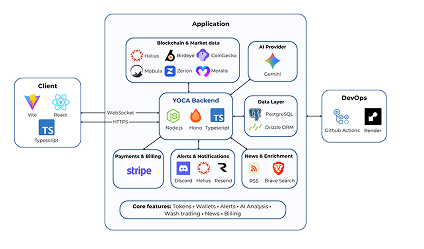
\includegraphics[width=1\textwidth]{images/arch.jpg}
    \caption{Kiến trúc tổng thể của hệ thống Yoca}
    \label{fig:kien_truc_tong_the}
\end{figure}

% Hình~\ref{fig:kien_truc_tong_the} nên thể hiện các thành phần chính gồm React frontend, Hono API backend, PostgreSQL, các domain service, các provider bên ngoài như Helius, Moralis, CoinGecko, Birdeye, Google Gemini, Stripe và Solana RPC. Ngoài ra, sơ đồ cũng nên làm rõ hướng dữ liệu đi từ frontend đến backend, từ backend đến cache, từ backend đến provider, sau đó quay lại frontend dưới dạng dữ liệu đã chuẩn hóa.


\subsection{Kiến trúc Monolith phân lớp và cơ chế Tải dữ liệu động (Lazy Loading)}

Trong phạm vi triển khai hiện tại, backend của Yoca được tổ chức theo hướng monolith phân lớp. Điều này có nghĩa là hệ thống backend được triển khai như một ứng dụng API thống nhất, nhưng bên trong được chia thành các lớp và miền nghiệp vụ riêng biệt. Các route chịu trách nhiệm tiếp nhận HTTP request và trả response. Các service chịu trách nhiệm xử lý nghiệp vụ. Các module tích hợp provider chịu trách nhiệm gọi API bên ngoài và chuẩn hóa dữ liệu. Lớp cơ sở dữ liệu chịu trách nhiệm định nghĩa schema, truy vấn và lưu trữ dữ liệu.

Cách tổ chức này phù hợp với quy mô của đồ án vì giúp hệ thống dễ triển khai, dễ kiểm thử và dễ theo dõi hơn so với việc tách thành nhiều microservices độc lập ngay từ đầu. Khi phát triển một sản phẩm có nhiều miền dữ liệu như token, ví, biểu đồ, AI, cảnh báo, thanh toán và hồ sơ người dùng, việc chia backend thành nhiều service vật lý có thể làm tăng độ phức tạp vận hành. Ngược lại, monolith phân lớp giúp nhóm tập trung vào việc hoàn thiện nghiệp vụ, đồng thời vẫn duy trì được cấu trúc module rõ ràng để có thể tách nhỏ trong tương lai nếu hệ thống phát triển lớn hơn.

Ở phía frontend, cơ chế tải dữ liệu động được áp dụng theo tương tác và ngữ cảnh sử dụng của người dùng. Thay vì tải toàn bộ dữ liệu ngay khi người dùng mở ứng dụng, mỗi trang hoặc thành phần giao diện chỉ gọi dữ liệu cần thiết cho chức năng hiện tại. Ví dụ, trang market chỉ cần dữ liệu thị trường và danh sách token, trang chi tiết token cần thêm dữ liệu lịch sử và biểu đồ, trong khi trang ví cần dữ liệu danh mục, giao dịch và lịch sử số dư. Cách tiếp cận này giúp giảm lượng dữ liệu tải ban đầu, cải thiện trải nghiệm người dùng và hạn chế số lượt gọi API không cần thiết.

Cơ chế tải dữ liệu động cũng phù hợp với đặc thù của dữ liệu blockchain. Một ví có thể có lịch sử giao dịch rất dài, nhưng người dùng không phải lúc nào cũng cần xem toàn bộ lịch sử đó ngay lập tức. Hệ thống có thể tải trước phần tổng quan, sau đó tải các phần chi tiết như giao dịch, swap hoặc biểu đồ số dư khi người dùng mở tab tương ứng. Cách làm này giúp phân bổ chi phí truy vấn theo nhu cầu thực tế, tránh gây tải lớn cho backend và provider bên ngoài.

\subsection{Chiến lược lưu trữ đệm (Caching) đa tầng}
% Rất quan trọng: Giải thích cơ chế TTL/window filtering cho dữ liệu ví, và on-conflict upserts cho dữ liệu thị trường (Token market/chart caches).

Caching là một trong những quyết định thiết kế quan trọng của Yoca. Dữ liệu on-chain và dữ liệu thị trường thường được lấy từ các nhà cung cấp bên thứ ba, trong khi các nhà cung cấp này có thể áp dụng giới hạn tần suất truy vấn, giới hạn gói sử dụng hoặc thay đổi độ trễ theo thời điểm. Nếu mỗi lần người dùng mở một trang hoặc thay đổi bộ lọc hệ thống đều gọi trực tiếp provider, ứng dụng sẽ dễ gặp lỗi rate limit, phản hồi chậm và khó kiểm soát chi phí. Vì vậy, hệ thống cần lưu trữ đệm dữ liệu đã lấy và tái sử dụng trong những trường hợp phù hợp.

Chiến lược caching của Yoca được thiết kế theo hướng ưu tiên cơ sở dữ liệu. Đối với các dữ liệu có thể tái sử dụng như lịch sử ví, danh mục tài sản, giao dịch, chuyển token, swap, dữ liệu biểu đồ và dữ liệu token, backend sẽ kiểm tra dữ liệu trong PostgreSQL trước. Nếu dữ liệu đã tồn tại và còn nằm trong ngưỡng hợp lệ, hệ thống trả về dữ liệu cache. Nếu dữ liệu chưa có hoặc không còn đủ mới, hệ thống gọi provider bên ngoài để đồng bộ phần dữ liệu cần thiết, sau đó chuẩn hóa và lưu lại vào cơ sở dữ liệu.

Đối với dữ liệu ví, caching cần quan tâm đến khái niệm khoảng thời gian dữ liệu đã được đồng bộ. Một ví có thể đã được đồng bộ lịch sử giao dịch cho một giai đoạn nhất định, nhưng chưa đầy đủ ở một giai đoạn khác. Vì vậy, hệ thống cần sử dụng metadata hoặc thông tin coverage để phân biệt phần dữ liệu đã có và phần dữ liệu còn thiếu. Cách tiếp cận này giúp hệ thống không phải tải lại toàn bộ lịch sử ví mỗi lần người dùng truy vấn, đồng thời vẫn đảm bảo khả năng bổ sung dữ liệu mới khi cần.

Đối với dữ liệu token và dữ liệu thị trường, hệ thống có thể sử dụng cơ chế TTL và ngưỡng cập nhật. Dữ liệu thị trường gần thời gian thực cần được cập nhật thường xuyên hơn, trong khi dữ liệu lịch sử cũ có thể được tái sử dụng lâu hơn. Khi nhận dữ liệu mới, backend có thể thực hiện upsert để cập nhật hoặc bổ sung bản ghi mà không tạo dữ liệu trùng lặp. Cách tiếp cận này giúp duy trì tập dữ liệu rolling ổn định cho các biểu đồ và bảng thống kê.

Caching không chỉ phục vụ hiệu năng mà còn giúp hệ thống ổn định hơn. Khi provider bên ngoài gặp lỗi tạm thời, dữ liệu cache có thể được sử dụng như một phương án dự phòng nếu vẫn còn phù hợp. Điều này đặc biệt quan trọng đối với các trang phân tích ví và biểu đồ, vì người dùng thường kỳ vọng hệ thống vẫn hiển thị được dữ liệu đã truy xuất trước đó thay vì báo lỗi hoàn toàn khi provider không phản hồi.



\subsection{Cơ chế đồng bộ hóa dữ liệu từ các nhà cung cấp (Helius, CoinGecko)}

Yoca tích hợp nhiều nhà cung cấp dữ liệu để phục vụ các miền nghiệp vụ khác nhau. Đối với dữ liệu ví Solana, hệ thống sử dụng Helius để truy xuất danh mục, lịch sử giao dịch, chuyển token và swap. Đối với dữ liệu thị trường và dữ liệu lịch sử giá token, hệ thống sử dụng CoinGecko. Ngoài ra, hệ thống còn có các đường tích hợp khác như Moralis cho một số luồng dữ liệu EVM hoặc dữ liệu dự phòng, Birdeye như một hướng fallback hoặc legacy path cho một số dữ liệu token, Google Gemini cho AI-assisted analysis, Stripe cho thanh toán và Solana RPC hoặc Helius RPC cho xác minh thanh toán on-chain.

Việc đồng bộ dữ liệu từ nhiều provider đòi hỏi backend phải có lớp chuẩn hóa dữ liệu. Mỗi provider có định dạng phản hồi, giới hạn truy vấn và cách biểu diễn dữ liệu khác nhau. Nếu frontend hoặc domain service phụ thuộc trực tiếp vào dữ liệu thô từ provider, hệ thống sẽ khó bảo trì và dễ bị ảnh hưởng khi provider thay đổi. Vì vậy, Yoca sử dụng các adapter hoặc service chuyên biệt để gọi provider, chuyển dữ liệu về DTO nội bộ và chỉ trả về định dạng đã được chuẩn hóa cho các lớp phía trên.

Đối với dữ liệu ví, luồng đồng bộ thường bắt đầu bằng việc người dùng nhập địa chỉ ví hoặc mở lại một ví đã từng phân tích. Backend kiểm tra metadata cache để xác định dữ liệu đã có. Nếu dữ liệu thiếu hoặc cần cập nhật, backend gọi provider để lấy dữ liệu mới theo từng loại như portfolio, transactions, transfers hoặc swaps. Sau đó, dữ liệu được chuẩn hóa, lưu vào các bảng cache tương ứng và trả về cho frontend. Cách tiếp cận này giúp hệ thống quản lý dữ liệu ví theo từng miền nhỏ thay vì xử lý toàn bộ dữ liệu ví như một khối đơn lẻ.

Đối với dữ liệu token, backend cần ánh xạ token address sang định danh phù hợp với nguồn dữ liệu giá. Đây là bước quan trọng vì mỗi provider có thể dùng khóa định danh khác nhau. Sau khi ánh xạ được token, hệ thống có thể lấy dữ liệu thị trường, dữ liệu giá lịch sử hoặc dữ liệu biểu đồ. Các dữ liệu này sau đó được lưu lại để phục vụ các lần truy vấn tiếp theo.

Cơ chế đồng bộ cũng cần xử lý lỗi và giới hạn truy vấn. Khi provider trả về lỗi 429 hoặc lỗi tạm thời, hệ thống cần có chính sách chờ, retry hoặc trả về dữ liệu cache nếu có. Khi nhiều API key được cấu hình, hệ thống có thể xoay vòng key để giảm nguy cơ gián đoạn. Những cơ chế này giúp hệ thống hoạt động ổn định hơn trong điều kiện phụ thuộc vào nhiều dịch vụ bên ngoài.



\section{Thiết kế chi tiết các luồng nghiệp vụ cốt lõi (Sequence Diagrams)}
\label{sec:thiet_ke_luong_nghiep_vu}

Phần này trình bày ba luồng nghiệp vụ cốt lõi của hệ thống: truy xuất và tổng hợp lịch sử giao dịch ví, truy vấn và trực quan hóa dữ liệu biểu đồ, và vấn đáp dữ liệu thông qua AI Assistant. Các luồng này đại diện cho những vấn đề kỹ thuật chính của Yoca, bao gồm truy xuất dữ liệu on-chain, sử dụng cache, chuẩn hóa dữ liệu, hiển thị biểu đồ và diễn giải dữ liệu.

\subsection{Luồng truy xuất và tổng hợp lịch sử giao dịch ví}

Luồng truy xuất và tổng hợp lịch sử giao dịch ví bắt đầu khi người dùng nhập một địa chỉ ví hoặc mở trang chi tiết ví. Frontend gửi yêu cầu đến backend thông qua service tương ứng. Backend tiếp nhận yêu cầu tại route ví, kiểm tra định dạng địa chỉ, xác định loại dữ liệu cần truy xuất và gọi wallet domain service.

Wallet service trước hết kiểm tra dữ liệu cache trong PostgreSQL. Nếu hệ thống đã có dữ liệu tổng quan, danh mục và lịch sử giao dịch còn phù hợp, service sẽ đọc dữ liệu từ cache và trả về cho route. Nếu cache chưa tồn tại hoặc chưa đủ dữ liệu cho khoảng thời gian người dùng yêu cầu, service gọi lớp fetcher để truy xuất dữ liệu từ provider bên ngoài. Dữ liệu nhận được từ provider được chuẩn hóa thành định dạng nội bộ, sau đó được lưu vào các bảng cache và metadata tương ứng.

Sau khi dữ liệu đã được chuẩn hóa, backend tổng hợp các thông tin cần thiết cho frontend. Các thông tin này có thể bao gồm danh sách token trong ví, giá trị ước tính, lịch sử giao dịch, giao dịch chuyển token, hoạt động swap và các thống kê tổng quan. Frontend nhận dữ liệu trả về, cập nhật trạng thái giao diện và hiển thị dữ liệu dưới dạng bảng hoặc biểu đồ.

% % TODO: Bổ sung sequence diagram cho luồng truy xuất ví.
% \begin{figure}[htbp]
% \centering
% \fbox{
% \begin{minipage}{0.85\textwidth}
% \centering
% \vspace{1.2cm}
% Sequence Diagram: Luồng truy xuất và tổng hợp lịch sử giao dịch ví \
% \textit{TODO: Chèn sơ đồ tuần tự tại đây.}
% \vspace{1.2cm}
% \end{minipage}
% }
% \caption{Luồng truy xuất và tổng hợp lịch sử giao dịch ví}
% \label{fig:lich_su_giao_dich}
% \end{figure}

% Hình~\ref{fig:lich_su_giao_dich} nên thể hiện các thành phần chính gồm User, React Frontend, Hono Route, Wallet Service, Cache Retriever, Provider Fetcher, PostgreSQL và Helius. Điểm cần nhấn mạnh trong sơ đồ là backend không gọi provider ngay lập tức trong mọi trường hợp, mà kiểm tra cache trước, sau đó chỉ gọi provider khi dữ liệu thiếu hoặc đã hết hạn.



\subsection{Luồng truy vấn và trực quan hóa biểu đồ (Chart Data Flow)}

Luồng truy vấn dữ liệu biểu đồ bắt đầu khi người dùng mở một trang có biểu đồ hoặc thay đổi tham số như token, ví, khoảng thời gian hoặc loại biểu đồ. Frontend gọi chart API thông qua service đã định nghĩa. Request gửi lên backend chứa các thông tin cần thiết để xác định loại biểu đồ, đối tượng phân tích và khoảng thời gian cần truy vấn.

Backend tiếp nhận request tại chart route. Tùy theo loại biểu đồ, route có thể gọi chart service, token service hoặc wallet service. Ví dụ, biểu đồ lịch sử giá token sẽ dựa nhiều vào dữ liệu token và dữ liệu thị trường, trong khi biểu đồ biến động số dư ví sẽ dựa vào dữ liệu ví và dữ liệu lịch sử số dư. Service tương ứng kiểm tra cache trước, sau đó gọi provider nếu dữ liệu chưa đủ hoặc cần cập nhật.

Dữ liệu biểu đồ sau khi được lấy từ cache hoặc provider sẽ được chuẩn hóa thành chuỗi thời gian. Mỗi điểm dữ liệu cần có mốc thời gian, giá trị và các metadata cần thiết để frontend có thể hiển thị. Đối với một số biểu đồ phức tạp, chẳng hạn biểu đồ số dư theo token hoặc biểu đồ giá trị danh mục, backend có thể cần kết hợp dữ liệu giao dịch với dữ liệu giá lịch sử để tính ra giá trị tại từng thời điểm.

Frontend nhận dữ liệu đã chuẩn hóa và truyền vào các component biểu đồ. Các component này chịu trách nhiệm hiển thị trục thời gian, đường dữ liệu, tooltip, chú thích, trạng thái tải dữ liệu và trạng thái lỗi. Cách tách biệt giữa backend xử lý dữ liệu và frontend hiển thị biểu đồ giúp hệ thống dễ mở rộng thêm loại biểu đồ mới mà không làm thay đổi quá nhiều cấu trúc tổng thể.

% % TODO: Bổ sung sequence diagram cho Chart Data Flow.
% \begin{figure}[htbp]
% \centering
% \fbox{
% \begin{minipage}{0.85\textwidth}
% \centering
% \vspace{1.2cm}
% Sequence Diagram: Luồng truy vấn và trực quan hóa biểu đồ \
% \textit{TODO: Chèn sơ đồ tuần tự tại đây.}
% \vspace{1.2cm}
% \end{minipage}
% }
% \caption{Luồng truy vấn và trực quan hóa dữ liệu biểu đồ}
% \label{fig:chart_data_flow}
% \end{figure}

% Hình~\ref{fig:chart_data_flow} nên thể hiện các thành phần gồm Chart Component, Chart API Client, Hono Chart Route, Chart Service, Token hoặc Wallet Service, PostgreSQL Cache và provider như CoinGecko hoặc Helius. Điểm cốt lõi của luồng là dữ liệu biểu đồ phải được chuẩn hóa trước khi trả về frontend để đảm bảo các component biểu đồ có thể tái sử dụng.

\subsection{Luồng vấn đáp dữ liệu thông qua AI Assistant}

Luồng vấn đáp thông qua AI Assistant bắt đầu khi người dùng đặt câu hỏi hoặc yêu cầu hệ thống phân tích một ví, một token hoặc một tập dữ liệu đã hiển thị. Frontend gửi câu hỏi cùng với ngữ cảnh cần thiết đến backend. Backend kiểm tra xác thực nếu chức năng yêu cầu người dùng đăng nhập, sau đó gọi service phụ trách wallet chat hoặc AI analysis.

Trước khi gọi mô hình AI, backend cần chuẩn bị ngữ cảnh dữ liệu. Đây là bước quan trọng vì AI không nên tự tạo ra số liệu hoặc tự suy đoán dữ liệu không có trong hệ thống. Service sẽ thu thập các chỉ số đã được tính toán, dữ liệu ví đã chuẩn hóa, dữ liệu token liên quan hoặc các kết quả phân tích có sẵn. Sau đó, backend chuyển các dữ liệu này thành một ngữ cảnh có cấu trúc để gửi đến mô hình AI.

Mô hình AI sử dụng ngữ cảnh đã chuẩn bị để tạo câu trả lời bằng ngôn ngữ tự nhiên. Câu trả lời có thể bao gồm tóm tắt danh mục ví, nhận xét về biến động tài sản, các giao dịch đáng chú ý hoặc giải thích một biểu đồ nhất định. Sau khi nhận kết quả, backend có thể lưu lại câu trả lời hoặc phiên chat nếu chức năng lưu lịch sử được bật. Frontend hiển thị câu trả lời trong giao diện chat hoặc trong vùng phân tích tương ứng.

% % TODO: Bổ sung sequence diagram cho AI Assistant.
% \begin{figure}[htbp]
% \centering
% \fbox{
% \begin{minipage}{0.85\textwidth}
% \centering
% \vspace{1.2cm}
% Sequence Diagram: Luồng vấn đáp dữ liệu thông qua AI Assistant \
% \textit{TODO: Chèn sơ đồ tuần tự tại đây.}
% \vspace{1.2cm}
% \end{minipage}
% }
% \caption{Luồng vấn đáp dữ liệu thông qua AI Assistant}
% \label{fig:ai_assistant}
% \end{figure}

% Hình~\ref{fig:ai_assistant} nên thể hiện các thành phần gồm User, Chat Component, Hono Route, Wallet Chat Service, PostgreSQL, AI Provider và giao diện trả kết quả. Điểm quan trọng cần thể hiện là AI chỉ nhận dữ liệu đã được backend chuẩn hóa và tóm tắt, thay vì truy cập trực tiếp vào dữ liệu thô hoặc tự tạo ra số liệu.


\input{Chapter3/database/database}

\section{Tiêu chí chấp nhận và phạm vi kiểm thử}
\label{sec:acceptance_plan}

Nhóm chúng em xác định tiêu chí chấp nhận theo các hành trình chính của người dùng. Các tiêu chí trong Bảng~\ref{tab:acceptance_criteria} liên kết yêu cầu chức năng với hành vi cần được duy trì khi hệ thống thay đổi; kết quả chạy các suite kiểm thử được trình bày tại Chương 5.

\small
\begin{longtable}{|p{3.1cm}|p{5.4cm}|p{6.0cm}|}
\caption{Kịch bản và tiêu chí chấp nhận các luồng chính}\label{tab:acceptance_criteria} \\
\hline
\textbf{Luồng} & \textbf{Kịch bản} & \textbf{Tiêu chí chấp nhận} \\
\hline
\endfirsthead
\hline
\textbf{Luồng} & \textbf{Kịch bản} & \textbf{Tiêu chí chấp nhận} \\
\hline
\endhead

Khám phá thị trường & Mở Market Overview, tìm token/pool/ví và chuyển giữa các trang liên quan & Kết quả dẫn đến đúng đối tượng; loading, empty và upstream error được hiển thị rõ; dữ liệu chính có đơn vị và thời điểm phù hợp \\
\hline
Token và pool & Mở token, xem chart/holder/pool rồi mở một pool và giao dịch gần đây & Address được giữ nhất quán qua các trang; biểu đồ và bảng không dùng dữ liệu sai schema; trường tùy chọn bị thiếu không làm hỏng toàn trang \\
\hline
Phân tích ví & Mở ví, thay khoảng thời gian, xem portfolio, PnL, balance, transfer và swap & Dữ liệu thuộc đúng ví và khoảng thời gian; danh sách lớn được phân trang/lọc; kết quả có giới hạn độ phủ phải được ghi rõ \\
\hline
So sánh và wash trading & So sánh nhiều ví; mở phân tích wash trading của một token và lần theo giao dịch liên quan & Các chỉ số dùng cùng định nghĩa; đồ thị liên kết được với dữ liệu nguồn; tín hiệu bất thường không được trình bày như kết luận chắc chắn \\
\hline
Tài khoản cá nhân & Đăng nhập, cập nhật profile, quản lý watchlist/label và thử truy cập dữ liệu của tài khoản khác & Thao tác hợp lệ được lưu; route bảo vệ từ chối request thiếu hoặc sai quyền; dữ liệu cá nhân không bị trả cho tài khoản khác \\
\hline
Cảnh báo & Tạo, sửa trạng thái và xóa cảnh báo token hoặc ví; tiếp nhận một sự kiện phù hợp & Rule được lưu đúng chủ sở hữu và điều kiện; sự kiện phù hợp được xử lý theo kênh hỗ trợ; lỗi provider không làm mất cấu hình cảnh báo \\
\hline
AI và subscription & Gửi câu hỏi có ngữ cảnh, quản lý session/prompt và sử dụng hết quota thử nghiệm & Phản hồi bám dữ liệu được cung cấp; lượt dùng được ghi nhận; chức năng bị khóa trả thông báo và hướng nâng gói rõ ràng \\
\hline
\end{longtable}
\normalsize

Phạm vi kiểm thử gồm các phép tính và normalizer, contract bằng fixture cho phản hồi provider, route/service với upstream được mock và component test cho trạng thái giao diện. Các ca kiểm thử tập trung vào validation, ownership, phân trang, dữ liệu nullable, chống ghi trùng, quota và cách hệ thống phản hồi khi dịch vụ bên ngoài trả lỗi. Cách tổ chức này bao phủ các ranh giới có ảnh hưởng trực tiếp đến dữ liệu hiển thị và những luồng nghiệp vụ chính trong Bảng~\ref{tab:acceptance_criteria}.

\section{Tổng kết chương}

Chương này đã chuyển mục tiêu chung của Yoca thành một hành trình sử dụng và các yêu cầu có thể đối chiếu. Khách có thể khám phá thị trường, token, pool, giao dịch và ví; người dùng đã đăng ký có thêm không gian cá nhân, cảnh báo, subscription và AI. So sánh ví và wash trading mở rộng luồng phân tích khi người dùng cần đối chiếu nhiều đối tượng hoặc quan sát quan hệ giao dịch.

Bên cạnh chức năng, nhóm chúng em đặt ra yêu cầu về khả năng kiểm chứng dữ liệu, xử lý lỗi, bảo vệ dữ liệu cá nhân và tính nhất quán của giao diện. Chương tiếp theo trình bày cách kiến trúc Yoca đáp ứng các yêu cầu trên trong điều kiện dữ liệu phụ thuộc nhiều provider.


\chapter{Kiến trúc và thiết kế hệ thống}
\label{Chapter4}

Chương này trình bày cách nhóm chúng em tổ chức Yoca từ giao diện, máy chủ API đến cơ sở dữ liệu và các nhà cung cấp bên ngoài. Nội dung tập trung vào ranh giới giữa các lớp, hợp đồng dữ liệu, cơ chế lưu đệm và những quyết định giúp hệ thống vận hành ổn định trong giới hạn của các API bên ngoài.

\section{Kiến trúc tổng thể}

Yoca là một ứng dụng web full-stack được quản lý trong cùng một monorepo. Phía người dùng sử dụng React và Vite; phía máy chủ là một ứng dụng Hono chạy trên Node.js, giao tiếp với client qua cả HTTPS lẫn WebSocket; dữ liệu có cấu trúc và cache bền vững được lưu trong PostgreSQL thông qua Drizzle ORM. Backend được triển khai như một monolith, nhưng mã nguồn được chia theo miền như token, pool, wallet, người dùng, cảnh báo, thanh toán và AI. Cách tổ chức này vừa đủ nhẹ cho quy mô nhóm, đồng thời tránh chi phí vận hành nhiều dịch vụ độc lập khi các chức năng vẫn chia sẻ lược đồ và dữ liệu.

\begin{figure}[H]
    \centering
    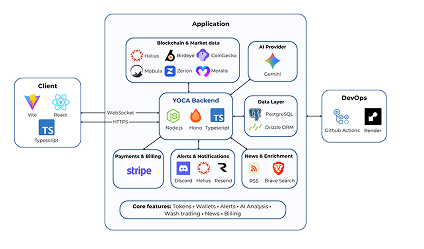
\includegraphics[width=\textwidth]{images/arch.png}
    \caption{Kiến trúc tổng thể và các phụ thuộc bên ngoài của hệ thống Yoca}
    \label{fig:system-architecture}
\end{figure}

Backend đóng vai trò trung chuyển duy nhất; giao diện chỉ trao đổi với API của Yoca. Các phụ thuộc bên ngoài gồm dữ liệu blockchain/thị trường (CoinGecko, Birdeye, Mobula, Zerion, Helius và Moralis), AI (Gemini), PostgreSQL, thanh toán (Stripe), cảnh báo/thông báo (Helius webhook, Resend và Discord) cùng tin tức/enrichment (RSS và Brave News). Khối DevOps nằm ngoài ranh giới \emph{Application} và thể hiện quan hệ build/deploy qua GitHub Actions và Render.

Ranh giới trung chuyển này đặc biệt quan trọng vì mỗi provider có cách biểu diễn token, thời gian, giá trị rỗng và phạm vi lịch sử riêng. Việc chuẩn hóa tại backend giữ những khác biệt đó khỏi các thành phần giao diện.

Các lớp được phân tách theo trách nhiệm nhưng vẫn nằm trong cùng một tiến trình backend. Route tiếp nhận và kiểm tra yêu cầu; service điều phối nghiệp vụ, provider và cache; lớp schema cùng repository quản lý dữ liệu bền vững. Cấu trúc theo miền giúp token, wallet, alert, payment và AI có thể phát triển độc lập về nghiệp vụ mà vẫn dùng chung hợp đồng và hạ tầng vận hành.

\section{Hợp đồng dữ liệu từ giao diện đến nhà cung cấp}

Ứng dụng dùng TypeScript ở cả client và server. Backend xuất kiểu của cây route Hono để client khởi tạo RPC client từ cùng một định nghĩa. Đường dẫn, tham số và kiểu phản hồi nhờ đó được kiểm tra xuyên suốt mà không cần sinh thêm mã từ một đặc tả trung gian. Hono phù hợp với quy mô của Yoca vì kết hợp định tuyến nhẹ với hợp đồng end-to-end trong cùng hệ sinh thái TypeScript \cite{hono}.

Hợp đồng kiểu ở thời điểm phát triển được bổ sung bằng validation runtime tại các biên hệ thống. Tham số từ người dùng và phản hồi của provider được kiểm tra bằng Zod trước khi đi vào phép tính hoặc cơ sở dữ liệu \cite{zod}. Các định danh như token address, wallet address và transaction signature được ràng buộc chặt; metadata hoặc chỉ số biến động được phép thiếu khi nguồn dữ liệu không bảo đảm giá trị. Cách xử lý fail-fast giúp hệ thống từ chối dữ liệu sai cấu trúc trước khi nó ảnh hưởng đến PnL, biểu đồ hoặc kết quả AI.

Lỗi được chuẩn hóa thành một response envelope gồm thông báo, mã lỗi và HTTP status phù hợp. Chi tiết nội bộ của provider không được chuyển nguyên văn ra giao diện; client chỉ cần ánh xạ các nhóm validation, authentication, entitlement, upstream và internal error sang trạng thái hiển thị tương ứng. Với dữ liệu cá nhân, user ID luôn lấy từ phiên xác thực và trở thành điều kiện của truy vấn. Chẳng hạn, thao tác đọc hoặc cập nhật Alert History đồng thời dùng định danh bản ghi và user ID, nhờ đó một tài khoản không thể truy cập lịch sử của tài khoản khác.

Hợp đồng này được áp dụng thống nhất từ route đến service và lớp lưu trữ: route xác nhận request, service trả dữ liệu nội bộ đã chuẩn hóa, còn database bảo vệ ownership cùng các khóa duy nhất. Thay đổi hình dạng response của provider vì vậy được giới hạn tại biên tích hợp.

\section{Luồng truy xuất, chuẩn hóa và lưu đệm}

Luồng truy xuất dữ liệu trước hết kiểm tra bản ghi đã lưu và thời điểm cập nhật. Dữ liệu còn hiệu lực được trả trực tiếp; dữ liệu thiếu hoặc hết hạn được lấy lại từ provider, kiểm tra cấu trúc, chuẩn hóa và ghi vào cơ sở dữ liệu trước khi phản hồi. Cùng một kiểu dữ liệu nội bộ vì vậy được duy trì ở cả hai nhánh, giúp route và giao diện không phụ thuộc vào hình dạng phản hồi của từng nguồn.

Mỗi provider được phân công theo miền dữ liệu phù hợp với thế mạnh và hạn mức sử dụng. CoinGecko và GeckoTerminal cung cấp dữ liệu thị trường, token và pool; Mobula đảm nhiệm PnL, lịch sử hoạt động và tổng giá trị tài sản của ví; Zerion cung cấp chuỗi số dư theo từng token; Helius bổ sung chi tiết giao dịch on-chain và sự kiện webhook. Birdeye và Moralis phục vụ một số tập dữ liệu chuyên biệt. Token metadata có thể được bổ sung từ nhiều nguồn khi cần, còn các phép phân tích chính sử dụng một nguồn ưu tiên để giữ kết quả nhất quán và dễ truy vết.

Cơ sở dữ liệu vừa lưu dữ liệu nghiệp vụ, vừa là lớp cache bền vững. Thiết kế bảng cân bằng mục tiêu chuẩn hóa với số lần gọi API cần thiết để hoàn thiện một bản ghi. Khi các phần dữ liệu có chu kỳ cập nhật khác nhau, chúng được tách thành bảng riêng để chỉ làm mới phần đã cũ. Thông tin hữu ích đi kèm response có thể bổ sung bảng liên quan sau khi đi qua khóa và ràng buộc nhất quán.

\input{Chapter3/database/database}

\section{Lựa chọn công nghệ và giới hạn của thiết kế}

React được chọn vì mô hình thành phần phù hợp với giao diện có nhiều bảng, biểu đồ và trạng thái tương tác dùng lại; Vite cung cấp máy chủ phát triển và cơ chế cập nhật mô-đun nhanh \cite{react,vite}. ECharts đảm nhiệm phần lớn biểu đồ tài chính \cite{echarts}, trong khi các cấu trúc quan hệ giao dịch cần một thành phần đồ thị tương tác riêng. Ở backend, Drizzle được chọn vì cách khai báo lược đồ gần với SQL và cho phép nhóm kiểm soát trực tiếp truy vấn, điều quan trọng khi cache và dữ liệu lịch sử cần các thao tác upsert hoặc truy vấn theo khoảng \cite{drizzle}.

Các lớp kiểm soát được bố trí theo từng ranh giới của hệ thống. Hono RPC duy trì hợp đồng giữa client và server; Zod kiểm tra dữ liệu ở runtime; các ràng buộc cơ sở dữ liệu bảo vệ trạng thái đã lưu; kiểm thử xác nhận hành vi kết hợp giữa các lớp. Cách tổ chức này giúp lỗi về đường dẫn, kiểu dữ liệu và phản hồi bên ngoài được phát hiện gần nơi phát sinh.

Ở phía giao diện, các trang được cấu thành từ lớp truy xuất dữ liệu, trạng thái tương tác và các thành phần trình bày dùng chung. Bảng, biểu đồ và đồ thị giao dịch nhận dữ liệu đã chuẩn hóa từ lớp nghiệp vụ, nhờ đó cùng một chỉ số có thể được sử dụng nhất quán ở Market, Token, Pool và Wallet. Trạng thái tải, dữ liệu rỗng và lỗi được biểu diễn theo cùng quy ước để người dùng luôn nhận biết được kết quả của thao tác.

Localization được tổ chức thành một lớp dùng chung cho nội dung và định dạng. Tiếng Anh và tiếng Việt sử dụng cùng hệ thống khóa; các formatter xử lý thống nhất số, phần trăm, đơn vị token, ngày giờ và tiền tệ. Dữ liệu tài chính được giữ ở đơn vị chuẩn trong API, sau đó lớp hiển thị mới áp dụng locale và quy đổi USD--VND. Thiết kế này hỗ trợ người dùng Việt Nam mà không làm thay đổi các phép tính nghiệp vụ.

\section{Ranh giới tin cậy và các điểm cần bảo vệ}

Yoca tiếp nhận dữ liệu và yêu cầu từ nhiều phía không đáng tin cậy như nhau: người dùng, ví Solana, webhook của provider và mô hình AI. Đăng nhập bằng ví yêu cầu người dùng ký một thông điệp chứa nonce dùng một lần; server xác minh chữ ký ed25519 khớp với public key trước khi cấp phiên đăng nhập, sau đó xóa nonce để tránh dùng lại. Với thanh toán, webhook Stripe được xác thực bằng chữ ký số của Stripe trước khi xử lý sự kiện, còn giao dịch thanh toán bằng Solana được backend truy vấn và đối chiếu địa chỉ nhận, số lượng cùng trạng thái xác nhận trước khi cấp quyền dịch vụ.

Webhook nhận sự kiện ví từ Helius được bảo vệ bằng thông tin xác thực trong header \texttt{Authorization}. Máy chủ kiểm tra thông tin này trước khi xử lý payload, đồng thời sử dụng khóa sự kiện để ngăn một lần gửi lại tạo ra cảnh báo hoặc bản ghi lịch sử trùng lặp.

Đối với AI, ngữ cảnh được xây dựng theo từng miền phân tích và tách khỏi lịch sử hội thoại cùng dữ liệu do công cụ trả về. Nội dung bên ngoài được đặt trong ranh giới rõ ràng để mô hình chỉ tuân theo hướng dẫn hệ thống; phản hồi sau đó được kiểm tra và chuẩn hóa cấu trúc trước khi trả về client. Dữ liệu cá nhân như watchlist, nhãn ví, cảnh báo và lịch sử thanh toán được giới hạn theo user ID đã xác thực như đã trình bày ở phần cơ sở dữ liệu.

\section{Kết chương}

Chương 4 đã xác định Yoca là một monolith phân lớp theo miền, có hợp đồng kiểu xuyên suốt giữa client và server, biên kiểm tra runtime cho dữ liệu bên ngoài và cơ chế lưu trữ ưu tiên tái sử dụng dữ liệu đã đồng bộ. Kiến trúc cân bằng giữa lược đồ chuẩn hóa, hạn mức API, tính nhất quán của dữ liệu và khả năng mở rộng theo miền nghiệp vụ. Trên nền thiết kế đó, Chương 5 trình bày cách hệ thống được triển khai, các chức năng chính và kết quả kiểm thử.


\chapter{Triển khai thực nghiệm và đánh giá}
\label{Chapter5}

Chương này trình bày cách Yoca được triển khai thành một hệ thống hoàn chỉnh, từ môi trường vận hành và quy trình tích hợp mã nguồn đến các chức năng người dùng và kết quả kiểm thử. Nội dung được tổ chức theo hành trình sử dụng của sản phẩm, qua đó cho thấy mối liên hệ giữa dữ liệu thị trường, token, pool, ví, cảnh báo và các mô-đun hỗ trợ phân tích.

\section{Môi trường, tích hợp và triển khai hệ thống}
\label{sec:moi_truong_trien_khai}

Yoca là một ứng dụng web full-stack được tổ chức trong npm workspace. Client sử dụng React 19 và Vite 7 để xây dựng giao diện; server vận hành trên Node.js với Hono để xử lý xác thực, nghiệp vụ và tích hợp dịch vụ. PostgreSQL lưu dữ liệu tài khoản, cấu hình người dùng và các cache bền vững; Drizzle ORM quản lý lược đồ cùng các truy vấn liên quan. ECharts đảm nhiệm phần lớn biểu đồ tài chính, trong khi quan hệ giao dịch giữa các ví được biểu diễn bằng đồ thị tương tác.

Dữ liệu được phân công theo miền chức năng. CoinGecko và GeckoTerminal cung cấp metadata, giá, lịch sử thị trường và dữ liệu pool; Birdeye bổ sung các nhóm dữ liệu giao dịch và xu hướng; Helius cung cấp danh mục ví, giao dịch đã giải mã và sự kiện webhook; Mobula đảm nhiệm các chỉ số phân tích ví cùng lịch sử tổng tài sản; Zerion cung cấp lịch sử ở cấp token; Moralis bổ sung metadata cho một số luồng. Gemini hỗ trợ diễn giải dữ liệu và Stripe phục vụ thanh toán thẻ. Các khóa truy cập, chuỗi kết nối và thông tin ký phiên chỉ được nạp ở server; client chỉ nhận những biến cấu hình công khai cần thiết cho quá trình build.

Mã nguồn client và server được quản lý trong cùng một Git repository. Workflow GitHub Actions chạy typecheck, lint, test và production build cho hai workspace. Các job được tách riêng để nhóm nhận biết nhanh lỗi thuộc hợp đồng kiểu, quy tắc mã nguồn, kiểm thử hay quá trình đóng gói. Khi toàn bộ bước kiểm tra trên nhánh \texttt{main} hoàn tất, job deploy kích hoạt hai Render deploy hook được lưu trong GitHub Actions Secrets.

Client và server được triển khai thành hai dịch vụ độc lập từ cùng monorepo. Render Static Site chạy Vite production build và phân phối thư mục \texttt{client/build}; Render Web Service build server rồi khởi động mã JavaScript bằng Node.js. Cơ sở dữ liệu PostgreSQL được vận hành trên Supabase. Cách tổ chức này cho phép hai thành phần có cấu hình và vòng đời triển khai riêng, đồng thời giữ lợi ích chia sẻ hợp đồng kiểu trong quá trình phát triển.

\begin{figure}[H]
    \centering
    \includegraphics[width=0.9\textwidth]{Chapter4/deployment-architecture.pdf}
    \caption{Kiến trúc tích hợp và triển khai của Yoca}
    \label{fig:deployment-architecture}
\end{figure}

Hình~\ref{fig:github-actions-ci} ghi nhận một lần chạy hoàn chỉnh của pipeline trên nhánh \texttt{main}. Sau bước kiểm tra, Render nhận revision mới và build hai dịch vụ. Giao diện được phục vụ tại \texttt{yoca.id.vn}; Web Service cung cấp API tại \texttt{yoca-backend.onrender.com} và kết nối đến cơ sở dữ liệu Supabase.

\begin{figure}[H]
    \centering
    \includegraphics[width=0.95\textwidth]{images/chapter5/github-actions-ci.png}
    \caption{Các job kiểm tra, build và deploy hoàn tất trên GitHub Actions}
    \label{fig:github-actions-ci}
\end{figure}

\begin{figure}[H]
    \centering
    \includegraphics[width=0.95\textwidth]{images/chapter5/render-deployment-frontend.jpg}
    \caption{Render Static Site phục vụ giao diện Yoca tại tên miền \texttt{yoca.id.vn}}
    \label{fig:render-deployment-frontend}
\end{figure}

\begin{figure}[H]
    \centering
    \includegraphics[width=0.95\textwidth]{images/chapter5/render-deployment-backend.jpg}
    \caption{Render Web Service vận hành API của Yoca}
    \label{fig:render-deployment-backend}
\end{figure}

\section{Kết quả triển khai các chức năng chính}
\label{sec:ket_qua_trien_khai}

Các chức năng của Yoca được kết nối theo một hành trình chung. Người dùng có thể bắt đầu từ dữ liệu thị trường, mở token hoặc pool liên quan, tiếp tục đến ví xuất hiện trong giao dịch, sau đó lưu đối tượng quan tâm hoặc thiết lập cảnh báo. Cách điều hướng này giữ ngữ cảnh phân tích và giúp các trang hỗ trợ lẫn nhau.

\subsection{Khám phá thị trường và tìm kiếm}

Market Overview tập hợp các nhóm dữ liệu như token thịnh hành, khối lượng và số giao dịch nổi bật, biến động giá, pool mới và hoạt động của các nhà giao dịch có lợi nhuận đáng chú ý. Người dùng lựa chọn khung thời gian, sắp xếp bảng và áp dụng bộ lọc về thanh khoản, vốn hóa, khối lượng hoặc độ tuổi pool. Mỗi kết quả là một điểm điều hướng đến token, pool hoặc ví tương ứng.

Thanh tìm kiếm toàn cục hỗ trợ token, pool và địa chỉ ví. Kết quả hiển thị các thông tin nhận diện cùng một số chỉ số chính, giúp người dùng phân biệt đối tượng trước khi mở trang chi tiết. Hai thành phần này tạo thành điểm bắt đầu của hành trình phân tích: Market Overview phục vụ khám phá, còn tìm kiếm đáp ứng nhu cầu truy cập một đối tượng đã biết.

\begin{figure}[H]
    \centering
    \includegraphics[width=0.95\textwidth]{images/chapter5/market-overview.png}
    \caption{Market Overview với nhóm Trending, bộ lọc thời gian và bảng token/pool}
    \label{fig:market-overview}
\end{figure}

\subsection{Phân tích token và pool}

Token Overview cung cấp thông tin nhận diện, giá, vốn hóa, khối lượng, nguồn cung và các mốc giá quan trọng. Biểu đồ hỗ trợ nhiều khoảng thời gian và cho phép người dùng quan sát giá, vốn hóa hoặc dữ liệu nến. Những nội dung chuyên sâu như phân bố holder, tokenomics, thị trường giao dịch và tin tức được tổ chức theo từng thẻ để người dùng mở rộng phân tích mà vẫn giữ nguyên token đang xem.

Phần holder kết hợp danh sách địa chỉ nắm giữ lớn với biểu đồ phân bố nguồn cung. Thông tin này giúp người dùng nhận biết mức độ tập trung tài sản và tiếp tục mở một địa chỉ ví để xem danh mục cùng lịch sử hoạt động. Tin tức và nội dung AI sử dụng token đang xem làm ngữ cảnh, nhờ đó phần diễn giải gắn với biểu đồ và dữ liệu thị trường được quan sát.

\begin{figure}[H]
    \centering
    \includegraphics[width=0.95\textwidth]{images/chapter5/token-overview.png}
    \caption{Thông tin thị trường và biểu đồ trên trang Token Overview}
    \label{fig:token-overview}
\end{figure}

\begin{figure}[H]
    \centering
    \includegraphics[width=0.85\textwidth]{images/chapter5/token-overview-holders.png}
    \caption{Danh sách holder và phân bố nguồn cung của token}
    \label{fig:token-overview-holders}
\end{figure}

Pool Detail tập trung vào một cặp giao dịch cụ thể. Trang hiển thị sàn giao dịch, địa chỉ pool, hai token thành phần, thanh khoản, khối lượng, biến động và lịch sử giao dịch gần nhất. Khi một token có nhiều pool, người dùng có thể chuyển pool để đối chiếu thanh khoản và diễn biến giao dịch. Biểu đồ nến phản ánh dữ liệu của pool đang chọn, bổ sung góc nhìn giao dịch thực tế cho các chỉ số tổng hợp ở Token Overview.

\begin{figure}[H]
    \centering
    \includegraphics[width=0.95\textwidth]{images/chapter5/token-pool.png}
    \caption{Thông tin thị trường và biểu đồ nến của pool đang được phân tích}
    \label{fig:token-pool}
\end{figure}

\subsection{Phân tích và so sánh ví}
\label{subsec:phan_tich_vi}

Wallet Overview tổng hợp danh mục tài sản, tổng giá trị ví, lịch sử số dư, PnL, win rate, khối lượng mua bán và mức độ hoạt động theo thời gian. Người dùng có thể thay đổi kỳ phân tích để quan sát sự khác biệt giữa các giai đoạn. Các biểu đồ về giá trị tài sản, phân bổ danh mục và kết quả giao dịch cung cấp góc nhìn tổng quan trước khi đi sâu vào từng token.

Mỗi vị thế token trình bày số dư, giá trị tại thời điểm truy vấn, lãi/lỗ đã thực hiện và đang ghi nhận, khối lượng mua bán, số lần giao dịch cùng giá mua và bán trung bình. Hoạt động của ví được chia thành swap và transfer; mỗi bản ghi giữ thời gian, tài sản, số lượng, địa chỉ liên quan và mã giao dịch. Khi người dùng mở chi tiết, Helius Enhanced Transactions cung cấp các lần chuyển token, chuyển SOL, chỉ thị thực thi và những tài khoản tham gia giao dịch.

\begin{figure}[H]
    \centering
    \includegraphics[width=0.95\textwidth]{images/chapter5/wallet-analysis.png}
    \caption{Tổng quan tài sản, PnL và hoạt động của một ví}
    \label{fig:wallet-analysis}
\end{figure}

\begin{figure}[H]
    \centering
    \includegraphics[width=0.9\textwidth]{images/chapter5/wallet-analysis-positions.png}
    \caption{Phân tích lãi/lỗ và hoạt động theo từng vị thế token}
    \label{fig:wallet-analysis-positions}
\end{figure}

Chức năng Compare Wallet cho phép chọn nhiều địa chỉ và đặt các chỉ số tổng hợp cạnh nhau. Bảng so sánh tập trung vào giá trị danh mục, PnL, win rate, khối lượng và số lượng giao dịch, phù hợp khi người dùng đã xác định được một nhóm ví cần đối chiếu. Đây là phần mở rộng của Wallet Overview nên sử dụng cùng cách tính và cùng kỳ phân tích, giúp kết quả giữa hai trang nhất quán.

\subsection{Tài khoản, theo dõi và cảnh báo}

Yoca hỗ trợ đăng nhập bằng email, Google và ví Solana. Người dùng đã xác thực có thể quản lý hồ sơ, liên kết ví, gắn nhãn địa chỉ, lưu watchlist, theo dõi gói dịch vụ và lịch sử thanh toán. Giao diện hỗ trợ tiếng Anh và tiếng Việt, đồng thời định dạng số, ngày giờ và giá trị tiền tệ theo locale được chọn.

Khi người dùng theo dõi một ví, hệ thống đồng bộ địa chỉ với Helius Webhook để nhận sự kiện mới. Quy tắc cảnh báo cho phép chọn loại sự kiện và điều kiện giá trị; thông báo được gửi qua email hoặc Discord theo cấu hình tài khoản. Mỗi sự kiện được lưu trong Alert History cùng nguồn, mức độ, trạng thái gửi và thời điểm. Người dùng có thể xem lịch sử, thay đổi trạng thái đọc; khóa sự kiện bảo đảm một lần gửi lại không tạo thêm bản ghi trùng lặp.

\begin{figure}[H]
    \centering
    \begin{minipage}{0.48\textwidth}
        \centering
        \includegraphics[width=\textwidth]{images/chapter5/alert-config-1.png}
    \end{minipage}
    \hfill
    \begin{minipage}{0.48\textwidth}
        \centering
        \includegraphics[width=\textwidth]{images/chapter5/alert-config-2.png}
    \end{minipage}
    \caption{Cấu hình điều kiện theo dõi hoạt động của ví}
    \label{fig:alert-config}
\end{figure}

\begin{figure}[H]
    \centering
    \includegraphics[width=0.85\textwidth]{images/chapter5/alert-delivery-email.png}
    \caption{Email cảnh báo được gửi khi giao dịch thỏa điều kiện theo dõi}
    \label{fig:alert-delivery-email}
\end{figure}

\subsection{Wash Trading và trợ lý AI}

Mô-đun Wash Trading tổ chức dữ liệu chuyển token thành đồ thị có hướng, trong đó mỗi nút biểu diễn một địa chỉ ví và mỗi cạnh biểu diễn một giao dịch chuyển token từ ví gửi đến ví nhận. Dữ liệu được thu thập, chuẩn hóa và phân tích tại máy chủ trước khi gửi đến giao diện. Để hạn chế chồng lấn trên đồ thị, các giao dịch có cùng chiều giữa một cặp ví được gộp thành một luồng; tổng lượng token và số lượt chuyển tương ứng được cộng dồn để người dùng dễ quan sát quan hệ giao dịch.

Hệ thống tìm kiếm các chu trình giao dịch nghi vấn và phân tích sáu đặc trưng của từng ví, gồm mức độ tham gia chu trình (\textit{circular pattern}), tín hiệu thời gian giao dịch (\textit{time regularity}), độ tương đồng lượng token (\textit{amount similarity}), giao dịch tự chuyển (\textit{self-loop}), mức độ kết nối của ví trong đồ thị (\textit{hubness}) và khối lượng tương đối so với ví có khối lượng lớn nhất (\textit{volume signal}). Trong đó, tín hiệu thời gian được xác định từ khoảng thời gian trung bình giữa các giao dịch liên tiếp; \textit{hubness} được tính dựa trên tổng số liên kết vào và ra của ví. Các đặc trưng được chuẩn hóa và tổng hợp bằng trọng số để tạo điểm nghi vấn cho từng ví, từ đó hỗ trợ người dùng tập trung vào các cấu trúc có dấu hiệu phối hợp, lặp lại hoặc luân chuyển token bất thường.

GCN, GAT và GraphSAGE trên giao diện là ba cấu hình trọng số heuristic lấy cảm hứng từ mạng nơ-ron đồ thị, không phải các mô hình GNN đã được huấn luyện trên dữ liệu có nhãn. GCN phân bổ trọng số tương đối cân bằng và ưu tiên tín hiệu chu trình; GAT tăng ảnh hưởng của chu trình và độ tương đồng lượng token; GraphSAGE tăng vai trò của \textit{hubness} và \textit{volume signal}. Việc chuyển đổi giữa ba cấu hình chỉ làm thay đổi mức đóng góp của các đặc trưng trong phép tính điểm rủi ro, qua đó cung cấp những góc nhìn phân tích khác nhau trên cùng một tập giao dịch. Trọng số và công thức tính cụ thể được trình bày tại Phụ lục~\ref{appendix:wash-trading-scoring}.

Kết quả phân tích bao gồm điểm rủi ro tổng thể của token, các chỉ số tổng hợp, đồ thị tương tác, danh sách ví nghi vấn, các chu trình nghi vấn được phát hiện, nhật ký phân tích và phần giải thích cho từng nhóm tín hiệu. Điểm rủi ro tổng thể được tổng hợp từ độ tin cậy của chu trình, điểm trung bình của các ví được giữ lại, tỷ lệ khối lượng liên quan đến các ví thuộc chu trình, tỷ lệ ví có mức rủi ro cao và mật độ ví nghi vấn trong toàn bộ đồ thị. Các kết quả này là tín hiệu hỗ trợ sàng lọc và không được xem là bằng chứng khẳng định một ví hoặc token đã thực hiện wash trading.

Trên đồ thị, người dùng có thể di chuột hoặc chọn một nút để xem địa chỉ, loại ví, trạng thái tham gia chu trình và điểm nghi vấn. Khi di chuột lên một cạnh, giao diện hiển thị ví gửi, ví nhận, tổng lượng token và số giao dịch đã được gộp.

Hình~\ref{fig:wash-trading-analysis} minh họa một phiên phân tích gồm 120 giao dịch của 69 ví. Giao diện tổng hợp điểm rủi ro, khối lượng giao dịch ước tính liên quan đến các ví thuộc chu trình, số ví cần chú ý và các cụm chu trình, sau đó biểu diễn luồng chuyển token để người dùng quan sát quan hệ giữa chúng. Khi chọn một ví, khu vực chi tiết hiển thị điểm nghi vấn cùng mức đóng góp của các đặc trưng \textit{circular pattern}, \textit{time regularity}, \textit{amount similarity}, \textit{self-loop}, \textit{hubness} và \textit{volume signal}. Cách trình bày này giúp người dùng đối chiếu điểm số với những tín hiệu đã tạo nên điểm và nhận biết nguyên nhân khiến một ví được đưa vào danh sách cần kiểm tra.

\begin{figure}[H]
    \centering
    \includegraphics[width=0.86\textwidth]{images/ui/wash-trading-1.png}

    \vspace{0.4em}
    \includegraphics[width=0.45\textwidth]{images/ui/wash-trading-2.png}
    \caption{Đồ thị giao dịch, cụm ví nghi vấn và điểm rủi ro của ví được chọn}
    \label{fig:wash-trading-analysis}
\end{figure}

Trợ lý AI hoạt động theo ngữ cảnh của từng khu vực phân tích. Tại trang Wash Trading, khung chat được giới hạn theo địa chỉ mint, khung thời gian, cấu hình chấm điểm và kết quả phân tích tương ứng. Trước khi gửi yêu cầu đến mô hình, máy chủ chuẩn bị ngữ cảnh gồm nguồn dữ liệu, các chỉ số tổng hợp, điểm rủi ro, chu trình nghi vấn, ví tiêu biểu, đặc trưng của ví và nhật ký phát hiện. Nhờ đó, trợ lý có thể giải thích nguyên nhân hình thành điểm, ý nghĩa của các đặc trưng, sự khác nhau giữa ba cấu hình chấm điểm và những tín hiệu đáng chú ý trong kết quả hiện tại.

Các tham số đầu vào của API được kiểm tra bằng schema Zod nhằm bảo đảm địa chỉ mint, khung thời gian, cấu hình thuật toán và nội dung câu hỏi đúng định dạng. Đối với phản hồi từ mô hình, máy chủ yêu cầu dữ liệu có cấu trúc JSON, sau đó thực hiện đọc và chuẩn hóa các trường cần thiết. Khi mô hình không khả dụng hoặc phản hồi không hợp lệ, hệ thống sử dụng phần phân tích cục bộ làm phương án thay thế để vẫn cung cấp thông tin cơ bản cho người dùng. Do đó, hệ thống không xem toàn bộ phản hồi AI là dữ liệu đã được xác thực trực tiếp bằng Zod, mà chỉ sử dụng các trường đã đọc và chuẩn hóa thành công.

Nguồn dữ liệu ưu tiên của mô-đun là Helius Enhanced Transactions; Helius RPC thông qua các tài khoản token được sử dụng như một phương án dự phòng. Khi không thể thu thập đủ dữ liệu on-chain, hệ thống có thể chuyển sang nguồn \texttt{demo-fallback}. Trong trường hợp này, giao diện và trợ lý sẽ thông báo rõ rằng kết quả chỉ là dữ liệu mô phỏng phục vụ minh họa quy trình và trải nghiệm người dùng, không phải kết luận được rút ra từ hoạt động on-chain thực tế.

Ngoài mô-đun Wash Trading, trợ lý AI còn được tích hợp tại Token Overview và Wallet Overview. Tại Token Overview, Ask Yoca AI sử dụng dữ liệu thị trường, biến động giá, thông tin holder và dữ liệu on-chain hiện có để giải thích xu hướng hoặc các tín hiệu rủi ro của token. Tại Wallet Overview, trợ lý sử dụng danh mục tài sản, vị thế token, lịch sử giao dịch và các chỉ số phân tích để giải thích hoạt động của ví. Hai trường hợp trong Hình~\ref{fig:yoca-ai-contexts} lần lượt minh họa phần phân tích rủi ro token và câu trả lời kết hợp nhận xét với biểu đồ số dư 30 ngày của ví đang được xem.

\begin{figure}[H]
    \centering
    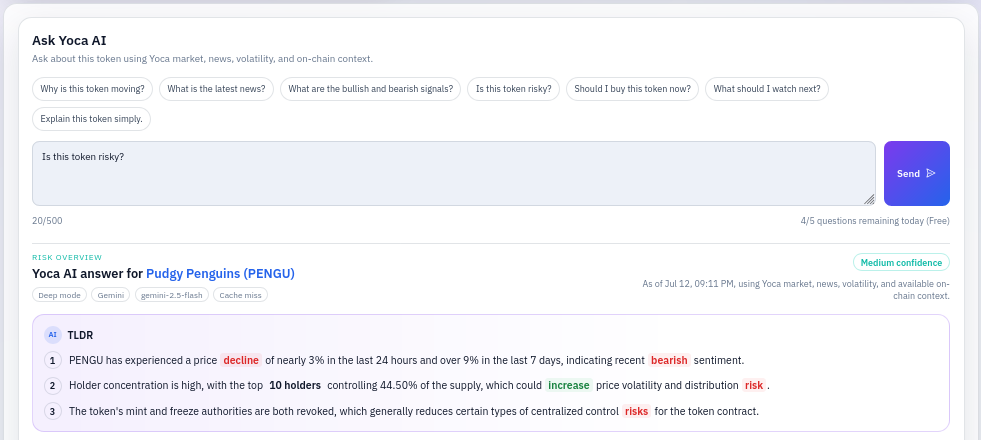
\includegraphics[width=0.88\textwidth]{images/ui/token_overview__ask_yoca_ai_is_this_token_risky.png}

    \vspace{0.4em}
    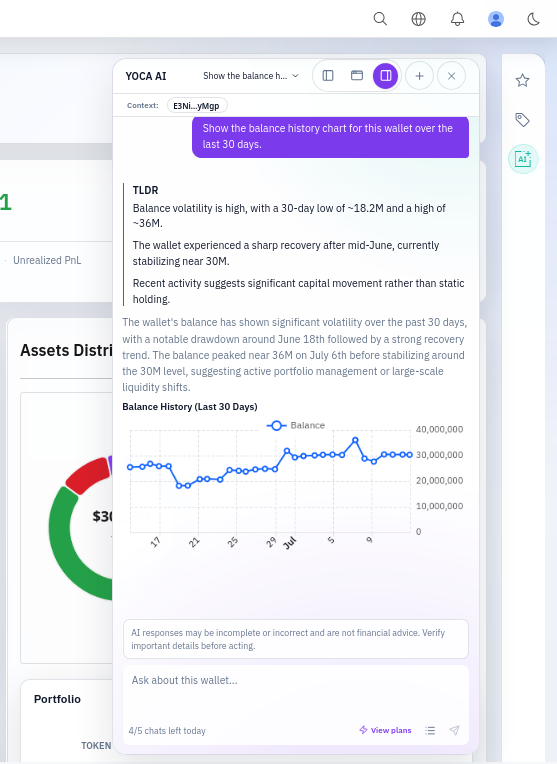
\includegraphics[width=0.46\textwidth]{images/ui/wallet_overview__wallet_ai_histrical_balance_30d.png}
    \caption{Ask Yoca AI phân tích token và Wallet AI giải thích lịch sử số dư 30 ngày}
    \label{fig:yoca-ai-contexts}
\end{figure}

\section{Các giải pháp kỹ thuật tiêu biểu}
\label{sec:giai_quyet_thach_thuc}

\subsection{Điều phối truy vấn và tái sử dụng dữ liệu}

Các provider áp dụng giới hạn theo số request, credit hoặc compute unit. Server đặt yêu cầu sau lớp điều phối theo từng dịch vụ và tái sử dụng dữ liệu đã lưu trước khi gọi ra ngoài. Với dữ liệu snapshot như metadata hoặc market overview, thời điểm cập nhật xác định dữ liệu còn hiệu lực. Với lịch sử giá, số dư, swap và transfer, metadata coverage ghi nhận khoảng đã đồng bộ; khi người dùng mở rộng thời gian, hệ thống chỉ tải phần còn thiếu rồi hợp nhất với dữ liệu trước đó.

Cơ chế này đặc biệt quan trọng với ví có lịch sử dài. Một yêu cầu mới có thể tái sử dụng phần lớn dữ liệu đã tải và chỉ cập nhật đoạn cuối gần thời điểm truy vấn. Các yêu cầu trùng nhau phát sinh đồng thời dùng chung kết quả đang xử lý, hạn chế việc nhiều thành phần giao diện cùng truy vấn một endpoint bên ngoài cho cùng đối tượng.

\subsection{Tổ chức dữ liệu cho phân tích ví}

Phân tích ví cần kết hợp nhiều lớp dữ liệu có ý nghĩa khác nhau. Mobula cung cấp chỉ số PnL, win rate, khối lượng và lịch sử tổng tài sản; Zerion cung cấp lịch sử ở cấp token; Helius cung cấp portfolio, giao dịch chi tiết và sự kiện on-chain. Server chuyển các phản hồi này về mô hình nội bộ, lưu theo địa chỉ cùng kỳ phân tích và cung cấp một contract thống nhất cho giao diện.

PnL tổng hợp phản ánh kết quả giao dịch theo dữ liệu phân tích của provider. Đường biến động theo ngày được xây dựng từ thay đổi tổng tài sản và dòng tiền vào/ra, giúp phân biệt biến động do hiệu quả tài sản với việc người dùng nạp hoặc rút tiền. Lịch sử theo token tiếp tục giữ mức chi tiết cần thiết để giải thích đóng góp của từng vị thế vào kết quả chung.

Helius Enhanced Transactions phục vụ lớp chi tiết giao dịch. Dữ liệu token transfer, native transfer, instruction và account change giúp người dùng đối chiếu hoạt động xuất hiện trong lịch sử swap hoặc transfer. Việc phân tách kết quả tổng hợp và dữ liệu chi tiết giữ cho trang Wallet phản hồi nhanh, đồng thời vẫn cung cấp đường dẫn về giao dịch nguồn.

\subsection{Kiểm soát dữ liệu và kết quả AI}

Phản hồi của provider được kiểm tra bằng schema trước khi đi vào phép tính hoặc cơ sở dữ liệu. Các định danh cốt lõi như token address, wallet address và transaction signature được ràng buộc chặt; metadata bổ sung được xử lý theo khả năng hiện diện của từng nguồn. Lỗi từ dịch vụ bên ngoài được chuyển về nhóm trạng thái thống nhất để giao diện hiển thị loading, empty hoặc error phù hợp.

Đối với AI, hướng dẫn hệ thống được tách khỏi câu hỏi, lịch sử hội thoại và dữ liệu do công cụ trả về. Chỉ những công cụ đã đăng ký mới được gọi; dữ liệu đầu vào được giới hạn theo miền đang phân tích. Mô hình trả kết quả theo cấu trúc xác định, sau đó server kiểm tra nội dung và ánh xạ citation về nguồn đã truy xuất. Nhờ đó, phần diễn giải luôn gắn với token, ví hoặc tập giao dịch đang được người dùng quan sát.

\section{Kết quả kiểm thử và đánh giá}
\label{sec:kiem_thu_danh_gia}

Yoca sử dụng Vitest ở cả client và server. Phía client kết hợp jsdom và Testing Library để kiểm tra component, thao tác người dùng, bảng, biểu đồ, hồ sơ, cảnh báo và thanh toán. Phía server kiểm tra route, service, xác thực, entitlement, payment, webhook, provider mapper, dữ liệu Wallet và các guardrail AI. Fixture và mock tạo ra các trường hợp dữ liệu hợp lệ, dữ liệu rỗng, tham số sai, vượt giới hạn truy vấn và lỗi dịch vụ bên ngoài.

Các test tập trung vào hành vi có khả năng ảnh hưởng trực tiếp đến kết quả hiển thị: kiểm tra ownership của dữ liệu người dùng, chống ghi trùng sự kiện cảnh báo, kết thúc phân trang, chuyển đổi response provider, xử lý trường nullable và từ chối phản hồi AI sai cấu trúc. Zod, hợp đồng TypeScript và ràng buộc PostgreSQL hỗ trợ kiểm tra dữ liệu ở các lớp khác nhau; test xác nhận hành vi khi những lớp này phối hợp trong route hoặc service.

\begin{table}[H]
\centering
\small
\begin{tabularx}{\textwidth}{|L{2.5cm}|C{2.2cm}|C{2.2cm}|X|}
\hline
\textbf{Suite} & \textbf{Test file} & \textbf{Test case} & \textbf{Phạm vi chính} \\
\hline
Client & 16/16 đạt & 178/178 đạt & Component, bảng và biểu đồ, payment, profile, Wallet và Alert History API. \\
\hline
Server & 29/29 đạt & 204/204 đạt & Auth và entitlement, payment, alert/webhook, provider mapping, Wallet, phân trang và AI guardrail. \\
\hline
\end{tabularx}
\caption{Kết quả kiểm thử client và server ngày 12/07/2026}
\label{tab:test_results}
\end{table}

Kết quả trong Bảng~\ref{tab:test_results} cho thấy các luồng nghiệp vụ chính đều có kiểm thử hồi quy và hai suite hoàn tất toàn bộ trường hợp đã định nghĩa. Pipeline CI chạy lại các suite cùng typecheck, lint và production build trước bước triển khai, giúp mỗi revision trên nhánh chính trải qua cùng một quy trình kiểm tra.

\section{Tổng kết chương}
\label{sec:tong_ket_ch4}

Chương 5 đã trình bày quá trình đưa kiến trúc Yoca thành một sản phẩm vận hành trên môi trường triển khai. Các chức năng Market, Token, Pool và Wallet tạo thành luồng phân tích cốt lõi; tài khoản, watchlist và cảnh báo duy trì quá trình theo dõi; Wash Trading và AI bổ sung khả năng phát hiện, trực quan hóa và diễn giải dữ liệu. Những chức năng này được hỗ trợ bởi lớp tích hợp provider, cơ chế tái sử dụng dữ liệu và hợp đồng thống nhất giữa client với server.

Kết quả kiểm thử và triển khai cho thấy hệ thống đáp ứng các nhóm chức năng đã xác định, từ xử lý dữ liệu đến tương tác người dùng. Trên cơ sở đó, Chương 6 tổng kết đóng góp của đề tài và trình bày các hướng mở rộng cho dữ liệu, mô-đun Wash Trading và trải nghiệm phân tích.


\chapter{Kết luận và Hướng phát triển}
\label{Chapter5}

Chương này tổng kết những kết quả chính của đề tài, đánh giá phạm vi mà Yoca đã giải quyết và trình bày các hướng phát triển có thể mở rộng giá trị của hệ thống. Các kết quả được xem xét trên cả hai phương diện: trải nghiệm phân tích dành cho người dùng và nền tảng kỹ thuật phục vụ việc thu thập, tổ chức và diễn giải dữ liệu Solana.

\section{Tổng kết các kết quả đạt được}

Yoca đã hình thành một hành trình phân tích liên tục từ thị trường đến dữ liệu ví. Người dùng có thể bắt đầu tại trang tổng quan để nhận biết token hoặc pool đáng chú ý, mở trang chi tiết để xem giá, thanh khoản, holder và giao dịch, sau đó tiếp tục đến các ví liên quan để quan sát danh mục tài sản và hành vi theo thời gian. Thanh tìm kiếm và các liên kết giữa những đối tượng giúp quá trình này diễn ra trong cùng một hệ thống, giữ được ngữ cảnh khi người dùng chuyển từ góc nhìn tổng quan sang dữ liệu chi tiết.

Phân tích ví là một trong những kết quả trọng tâm của đề tài. Yoca tổng hợp giá trị danh mục, lịch sử số dư, khối lượng giao dịch, PnL và các vị thế token theo nhiều khoảng thời gian. Lịch sử swap và transfer được chuẩn hóa để người dùng theo dõi hoạt động của ví và mở chi tiết từng giao dịch khi cần đối chiếu. Chức năng so sánh nhiều ví bổ sung góc nhìn tương quan giữa hiệu quả, mức độ hoạt động và cơ cấu tài sản, qua đó hỗ trợ việc nhận biết những khác biệt đáng chú ý giữa các địa chỉ.

Mô-đun Wash Trading mở rộng phạm vi phân tích từ từng giao dịch sang cấu trúc quan hệ giữa nhiều ví. Dữ liệu chuyển token được biểu diễn bằng đồ thị có hướng; mỗi cạnh thể hiện luồng chuyển từ ví gửi đến ví nhận và có thể được gộp theo cùng chiều giữa một cặp ví để giảm chồng lấn khi hiển thị. Các đặc trưng về chu trình, khoảng thời gian trung bình giữa các giao dịch liên tiếp, độ tương đồng lượng token, self-loop, hubness và khối lượng tương đối được kết hợp để tạo điểm nghi vấn cho ví và điểm rủi ro tổng thể của token. Kết quả được trình bày cùng đồ thị, danh sách ví nghi vấn và các chu trình nghi vấn, giúp người dùng quan sát cơ sở hình thành tín hiệu trước khi tiếp tục đối chiếu dữ liệu giao dịch.

Trợ lý AI được tích hợp vào các miền token, ví và Wash Trading để diễn giải dữ liệu theo ngữ cảnh. Máy chủ chuẩn bị các chỉ số và dữ liệu liên quan trước khi gửi yêu cầu đến mô hình; các tham số đầu vào được kiểm tra bằng schema, còn phản hồi từ mô hình được yêu cầu ở dạng JSON để đọc và chuẩn hóa các trường cần thiết. Riêng với Wash Trading, ngữ cảnh gồm mint, khung thời gian, cấu hình chấm điểm và kết quả phân tích hiện tại; khi mô hình không khả dụng hoặc phản hồi không hợp lệ, hệ thống sử dụng phần phân tích cục bộ làm phương án thay thế. Các chức năng watchlist, nhãn ví và cảnh báo hỗ trợ người dùng lưu lại đối tượng quan tâm, theo dõi sự kiện và duy trì quá trình phân tích qua nhiều lần sử dụng. Giao diện tiếng Việt cùng cách trình bày số, ngày giờ và giá trị quy đổi giúp hệ thống gần gũi hơn với người dùng trong nước.

Ở lớp kỹ thuật, Yoca xây dựng một mô hình tích hợp dữ liệu theo miền. CoinGecko, GeckoTerminal và Birdeye cung cấp dữ liệu thị trường; Helius phục vụ danh mục ví, giao dịch và sự kiện on-chain; Mobula cung cấp các chỉ số phân tích ví và lịch sử tổng tài sản; Zerion đảm nhiệm lịch sử ở cấp token; Moralis bổ sung metadata cho một số luồng dữ liệu. Các nguồn này được đặt sau lớp kiểm tra và chuẩn hóa chung, nhờ đó phần giao diện không phụ thuộc trực tiếp vào cấu trúc phản hồi riêng của từng dịch vụ.

Cơ sở dữ liệu vừa lưu thông tin nghiệp vụ, vừa tái sử dụng dữ liệu đã đồng bộ. Dữ liệu dạng snapshot được quản lý theo thời gian hiệu lực, còn lịch sử giao dịch và số dư được theo dõi theo khoảng đã tải. Cách tổ chức này giảm số lần truy vấn lặp, hỗ trợ phân trang dữ liệu dài và cho phép từng nhóm thông tin được cập nhật theo nhịp riêng. Hợp đồng kiểu giữa client và server, kiểm tra dữ liệu ở runtime và các ràng buộc trong PostgreSQL tạo thành nhiều lớp bảo vệ cho quá trình trao đổi và lưu trữ dữ liệu.

Đề tài cũng hoàn thiện quy trình kiểm tra và triển khai sản phẩm. Các bộ kiểm thử phía client và server bao phủ những miền quan trọng như xác thực, thanh toán, cảnh báo, dữ liệu ví, provider adapter và AI. Lần chạy được ghi nhận trong báo cáo đạt 178/178 test phía client và 204/204 test phía server. GitHub Actions thực hiện typecheck, lint, test và production build trước khi kích hoạt quá trình triển khai. Giao diện và máy chủ được vận hành thành hai dịch vụ độc lập trên Render, kết nối với PostgreSQL trên Supabase và phục vụ tại tên miền của Yoca.

\section{Giới hạn của đề tài}

Khả năng phân tích của Yoca chịu ảnh hưởng bởi độ phủ dữ liệu từ các dịch vụ bên ngoài. Token mới, tài sản có thanh khoản thấp hoặc giao dịch có cấu trúc phức tạp có thể thiếu metadata, giá lịch sử hoặc thông tin dẫn xuất cần thiết. Quota và phạm vi lịch sử của từng nhà cung cấp cũng tác động đến tần suất cập nhật. Hệ thống sử dụng cache, kiểm tra dữ liệu và phân công nguồn theo từng miền để duy trì kết quả nhất quán trong phạm vi dữ liệu nhận được.

Các chỉ số PnL, nội dung AI và điểm Wash Trading được sử dụng như công cụ hỗ trợ phân tích. Giá trị của chúng phụ thuộc vào khoảng thời gian, dữ liệu giá và tập giao dịch được quan sát. Đối với Wash Trading, các đặc trưng và trọng số chỉ làm nổi bật các cấu trúc có dấu hiệu bất thường trên đồ thị; người dùng cần đối chiếu thêm giao dịch gốc, bối cảnh thị trường và nguồn dữ liệu liên quan trước khi đưa ra nhận định cuối cùng. Kết quả từ nguồn demo-fallback chỉ minh họa luồng giao diện và không được xem là kết luận từ dữ liệu on-chain thật. Hoạt động đánh giá của đề tài tập trung vào tính đúng đắn của luồng xử lý và các chức năng cốt lõi.

Ngoài kết quả về chức năng, đề tài đã giải quyết các vấn đề quan trọng khi làm việc với dữ liệu Web3. Cơ chế điều phối yêu cầu, luân phiên khóa truy cập và thử lại có kiểm soát giúp hạn chế tác động của giới hạn truy vấn. Chiến lược lưu đệm theo phạm vi thời gian cho phép tái sử dụng dữ liệu đã có và chỉ truy xuất phần còn thiếu. Đối với giá trị danh mục lịch sử, hệ thống tái dựng số dư tại từng thời điểm và kết hợp với dữ liệu giá tương ứng, qua đó tạo cơ sở cho biểu đồ số dư và PnL.

Hướng phát triển đầu tiên là mở rộng chiều sâu của dữ liệu và khả năng theo dõi chất lượng nguồn. Khi hệ thống phục vụ nhiều người dùng hơn, các chỉ số về thời gian phản hồi, tỷ lệ lỗi, mức sử dụng quota và hiệu quả cache có thể được tổng hợp để điều chỉnh chiến lược cập nhật theo từng provider. Dữ liệu lịch sử cũng có thể được lưu trữ theo các lớp thời gian phù hợp với nhu cầu truy vấn, giúp các phân tích dài hạn duy trì tốc độ phản hồi ổn định.

Đối với Wash Trading, hệ thống có thể bổ sung tập dữ liệu được gán nhãn và mở rộng thực nghiệm trên nhiều token, pool cùng giai đoạn thị trường khác nhau. Các đặc trưng hiện có tạo nền tảng cho việc đánh giá thêm những yếu tố như biến động giá, thay đổi thanh khoản, tần suất lặp lại giữa các cụm ví và hành vi qua nhiều pool. Khi dữ liệu đánh giá đủ lớn, các cấu hình GCN, GAT và GraphSAGE có thể được phát triển từ bộ trọng số heuristic hiện tại thành mô hình học trên đồ thị hoặc được hiệu chỉnh bằng phương pháp thống kê để tăng độ tin cậy của kết quả.

Các chức năng AI có thể tăng khả năng giải thích bằng cách liên kết từng nhận định với giao dịch, vị trí trên biểu đồ hoặc chỉ số đã sử dụng. Điều này giúp người dùng chuyển trực tiếp từ phần diễn giải đến dữ liệu cần kiểm tra. Cùng với đó, Yoca có thể mở rộng không gian cá nhân thành một quy trình nghiên cứu hoàn chỉnh hơn, nơi watchlist, nhãn ví, cảnh báo và lịch sử phân tích được kết nối theo từng chủ đề mà người dùng quan tâm.

Nhìn chung, đề tài đã xây dựng được một nền tảng phân tích dữ liệu Solana có luồng sử dụng rõ ràng, kết hợp dữ liệu thị trường với phân tích ví, giao dịch và quan hệ đồ thị. Quá trình thực hiện giúp nhóm chúng em giải quyết đồng thời các bài toán tích hợp nhiều nguồn, quản lý dữ liệu lịch sử, trực quan hóa thông tin và hỗ trợ diễn giải kết quả. Những thành phần đã xây dựng tạo cơ sở để Yoca tiếp tục phát triển thành một công cụ phân tích on-chain có chiều sâu và phù hợp hơn với nhu cầu của người dùng Việt Nam.


\addcontentsline{toc}{chapter}{Tài liệu tham khảo}

\DeclareNameAlias{sortname}{family-given}
\DeclareNameAlias{default}{family-given}

\printbibliography[title={Tài liệu tham khảo}]

\appendix

\chapter{Phương pháp tính điểm Wash Trading}
\label{appendix:wash-trading-scoring}

Phụ lục này trình bày cách mô-đun Wash Trading chuyển dữ liệu giao dịch thành các đặc trưng trên đồ thị và tổng hợp chúng thành điểm rủi ro. Mục đích của phần trình bày là làm rõ ý nghĩa của kết quả trên giao diện và cho phép người đọc lần theo các thành phần tạo nên điểm số. Các cấu hình GCN, GAT và GraphSAGE trong Yoca là ba bộ trọng số heuristic lấy cảm hứng từ cách quan sát cấu trúc lân cận của mạng nơ-ron đồ thị; hệ thống không sử dụng một mô hình GNN đã huấn luyện.

\section{Dữ liệu đầu vào và biểu diễn đồ thị}

Mỗi bản ghi đầu vào gồm địa chỉ ví gửi, địa chỉ ví nhận, lượng token đã quy đổi theo số chữ số thập phân, thời điểm giao dịch, địa chỉ mint và chữ ký giao dịch. Với một token và khoảng thời gian được chọn, Yoca chuẩn hóa các bản ghi thành đồ thị có hướng $G=(V,E)$. Mỗi đỉnh $v\in V$ biểu diễn một ví, còn mỗi cạnh $e=(u,v)\in E$ biểu diễn một lần chuyển token từ ví $u$ đến ví $v$. Lượng token và thời điểm được giữ như thuộc tính của cạnh.

Cách biểu diễn này cho phép hệ thống xem xét đồng thời hành vi của từng ví và quan hệ giữa nhiều ví. Một chu trình được tìm bằng phép duyệt theo chiều sâu trên các ví có hoạt động nổi bật. Đường đi hợp lệ gồm từ ba đến sáu bước, lượng token của từng cạnh lệch không quá 12\% so với cạnh khởi đầu và khoảng thời gian giữa các bước liên tiếp không vượt quá hai giờ. Gọi $\delta$ là tỷ lệ chênh lệch lượng token khi đóng vòng và $\overline{\Delta t}_{cycle}$ là khoảng thời gian trung bình giữa các bước, độ tin cậy của chu trình được tính bởi

\begin{equation}
p_{cycle}=\min\left(0{,}98,\max\left(0{,}45,
1-3{,}2\delta-\frac{\max(0,\overline{\Delta t}_{cycle}-90000)}{900000}\right)\right).
\end{equation}

Các chu trình trùng tập ví được hợp nhất, sau đó hệ thống giữ tối đa 20 chu trình có độ tin cậy cao nhất để trình bày.

\section{Các đặc trưng của ví}

Với mỗi ví $v$, hệ thống tính sáu đặc trưng đã chuẩn hóa về đoạn $[0,1]$. Ký hiệu $\operatorname{clip}(x)=\min(1,\max(0,x))$.

\textbf{Mức tham gia chu trình.} Nếu ví xuất hiện trong ít nhất một chu trình, đặc trưng $c_v$ nhận giá trị $0{,}94$; các trường hợp còn lại nhận giá trị 0. Giá trị nhỏ hơn 1 dành khoảng cho những tín hiệu bổ sung trong phép tổng hợp.

\textbf{Khoảng cách thời gian.} Các thời điểm liên quan đến ví được sắp xếp tăng dần. Với khoảng cách trung bình $\overline{\Delta t}$ tính bằng mili giây, đặc trưng thời gian được xác định bởi

\begin{equation}
t_v=\operatorname{clip}\left(1-\frac{\overline{\Delta t}}{900000}\right).
\end{equation}

Đặc trưng này được sử dụng khi có ít nhất ba khoảng thời gian liên tiếp. Giao dịch càng gần nhau thì $t_v$ càng lớn.

\textbf{Độ tương đồng lượng token.} Gọi $\mu_v$ và $\sigma_v$ lần lượt là trung bình và độ lệch chuẩn của lượng token trong các giao dịch liên quan đến ví. Khi có ít nhất ba quan sát và $\mu_v>0$, hệ thống tính

\begin{equation}
a_v=\operatorname{clip}\left(1-\frac{\sigma_v}{\mu_v}\right).
\end{equation}

Giá trị gần 1 cho biết lượng token giữa các giao dịch tương đối giống nhau.

\textbf{Self-loop.} Đặc trưng $s_v$ nhận giá trị $0{,}85$ khi tồn tại cạnh từ ví về chính nó và nhận giá trị 0 trong trường hợp còn lại.

\textbf{Hubness.} Gọi $d_v=d_v^{in}+d_v^{out}$ là tổng bậc vào và bậc ra, còn $d_{max}$ là bậc lớn nhất trong đồ thị đang xét. Mức độ kết nối tương đối của ví được tính bằng

\begin{equation}
h_v=\min\left(1,\frac{d_v}{\max(1,d_{max})}\right).
\end{equation}

\textbf{Khối lượng tương đối.} Với $q_v$ là tổng lượng token đi qua ví và $q_{max}$ là giá trị lớn nhất trong tập đang phân tích, đặc trưng khối lượng là

\begin{equation}
q'_v=\min\left(1,\frac{q_v}{\max(1,q_{max})}\right).
\end{equation}

Hai đặc trưng cuối mang ý nghĩa tương đối trong tập giao dịch được chọn. Chúng giúp nhận biết ví có vai trò nổi bật trong cấu trúc đang phân tích mà không quy đổi lượng token sang giá trị tiền tệ.

\section{Điểm rủi ro của ví}

Điểm của một ví là tổng có trọng số của sáu đặc trưng:

\begin{equation}
r_v=\min\left(0{,}97,
w_c c_v+w_t t_v+w_a a_v+w_s s_v+w_h h_v+w_q q'_v\right).
\end{equation}

Ba cấu hình trên giao diện khác nhau ở mức độ ưu tiên dành cho từng đặc trưng. Bảng~\ref{tab:wash-trading-weights} trình bày các trọng số đang được sử dụng.

\begin{table}[H]
    \centering
    \caption{Trọng số của ba cấu hình tính điểm Wash Trading}
    \label{tab:wash-trading-weights}
    \begin{tabular}{lccc}
        \hline
        \textbf{Đặc trưng} & \textbf{GCN} & \textbf{GAT} & \textbf{GraphSAGE} \\
        \hline
        Tham gia chu trình & 0,32 & 0,36 & 0,24 \\
        Khoảng cách thời gian & 0,21 & 0,17 & 0,18 \\
        Độ tương đồng lượng token & 0,21 & 0,27 & 0,17 \\
        Self-loop & 0,06 & 0,05 & 0,06 \\
        Hubness & 0,14 & 0,10 & 0,25 \\
        Khối lượng tương đối & 0,06 & 0,05 & 0,10 \\
        \hline
        \textbf{Tổng} & \textbf{1,00} & \textbf{1,00} & \textbf{1,00} \\
        \hline
    \end{tabular}
\end{table}

Cấu hình GCN phân bổ trọng số tương đối cân bằng và ưu tiên chu trình. GAT tăng ảnh hưởng của chu trình cùng độ tương đồng lượng token. GraphSAGE dành trọng số lớn hơn cho hubness và khối lượng, phù hợp khi cần quan sát vai trò của một ví trong vùng lân cận. Ví có điểm dưới $0{,}22$ và không tham gia chu trình được lược khỏi danh sách cần chú ý. Các mức Low, Medium và High lần lượt tương ứng với $r_v<0{,}45$, $0{,}45\leq r_v<0{,}72$ và $r_v\geq0{,}72$.

\section{Điểm tổng hợp của tập giao dịch}

Điểm rủi ro chung kết hợp năm tín hiệu: độ tin cậy của các chu trình ($C$), điểm trung bình của các ví được giữ lại ($R$), tỷ lệ khối lượng liên quan đến ví nằm trong chu trình ($W$), tỷ lệ ví mức High trong danh sách nghi vấn ($H$) và mật độ ví nghi vấn so với toàn bộ đồ thị ($D$). Với $P$ là tập chu trình, $S$ là danh sách ví nghi vấn, $V$ là tập ví và $S_H$ là tập ví mức High, các tín hiệu được tính như sau:

\begin{align}
C &= \min\left(1,\frac{\sum_{p\in P}p_{cycle}}{4}\right),
& R &= \frac{\sum_{v\in S}r_v}{|S|}, \\
W &= \min\left(1,\frac{\text{tỷ lệ khối lượng liên quan chu trình}}{75\%}\right),
& H &= \frac{|S_H|}{|S|}, \\
D &= \min\left(1,\frac{2|S|}{|V|}\right). &&
\end{align}

Khi mẫu số của một tỷ lệ bằng 0, tín hiệu tương ứng nhận giá trị 0. Các đại lượng được giới hạn trong đoạn $[0,1]$ trước khi tổng hợp:

\begin{align}
Z &= 0{,}30C+0{,}25R+0{,}20W+0{,}15H+0{,}10D, \\
R_{overall} &= \min\left(98,\operatorname{round}(100Z)\right).
\end{align}

Kết quả được hiển thị trên thang 100 điểm. Các khoảng dưới 20, từ 20 đến 44, từ 45 đến 74 và từ 75 trở lên lần lượt tạo các nhãn Clean, Low Risk, Medium Risk và High Risk. Bên cạnh điểm tổng, giao diện giữ lại đồ thị, chu trình, ví liên quan và mức đóng góp của từng đặc trưng. Nhờ đó, điểm số đóng vai trò định hướng vùng dữ liệu cần xem xét và luôn đi kèm thông tin giúp người dùng kiểm tra giao dịch nguồn.


\end{document} 
